\part{Graph and Network Theory}
	\chapter{Graphs and Subgraphs}
		\section{Graph}
			\begin{definition}[Graph]
				A \textbf{graph} G consists of a finite set $V(G)$ on vertices, a finite set $E(G)$ on edges and an \textbf{incident relation} than associates with any edge $e\in E(G)$ an unordered pair of vertices not necessarily distinct called \textbf{ends}.
			\end{definition}

			\begin{example}
				The following graph

				\begin{figure}[!h]
					\centering
					\begin{tikzpicture}[node distance = 1.3cm]
						\node (v_2) [solidNode, label=above:{$v_2$}] {};
						\node (v_3) [solidNode, label=above:{$v_3$}, right of = v_2] {};
						\node (v_1) [solidNode, label=below:{$v_1$}, below of = v_2] {};
						\node (v_4) [solidNode, label=below:{$v_4$}, below of = v_3] {};
						\node (v_5) [solidNode, label=above:{$v_5$}, right of = v_3] {};
						\node (v_6) [solidNode, label=below:{$v_6$}, below of = v_5] {};
						\draw [link] (v_2) -- node [left] {$e_2$} (v_1);
						\draw [link] (v_2) -- node [below] {$e_5$} (v_4);
						\draw [link] (v_1) to [out = 180, in = 270, looseness = 5] node [left] {$e_1$} (v_1);
						\draw [link] (v_2) to [out = 45, in = 135] node [above] {$e_3$} (v_3);
						\draw [link] (v_2) -- node [below] {$e_4$} (v_3);
						\draw [link] (v_3) -- node [right] {$e_6$} (v_1);
						\draw [link] (v_5) -- node [right] {$e_7$} (v_6);
					\end{tikzpicture}
				\end{figure}
				can be represented as\\
				\begin{align}
					V &= V(G) = \{v_1, v_2, v_3, v_4, v_5, v_6\} \\
					E &= E(G) = \{e_1, e_2, e_3, e_4, e_5, e_6, e_7\}\\
					e_1 &= v_1v_2, \quad e_2 = v_2v_4, \quad \dots
				\end{align}
			\end{example}

			\begin{definition}[Loop, Parallel, Simple Graph]
				An edge with identical ends is called a \textbf{loop}, Two edges having the same ends are said to be \textbf{parallel}, A graph without loops or parallel edges is called \textbf{simple graph}
			\end{definition}

			\begin{definition}[Adjacent]
				Two edges of a graph are \textbf{adjacent} if they have a common end, two vertices are \textbf{adjacent} if they are jointed by an edge.
			\end{definition}

		\section{Graph Isomorphism}

		\section{The Adjacency and Incidence Matrices}

		\section{Subgraph}
			\begin{definition}[Subgraph]
				Given two graphs $G$ and $H$, $H$ is a \textbf{subgraph} of $G$ if $V(H)\subseteq V(G)$, $E(H)\subseteq E(G)$ and an edge has the same ends in $H$ as it does in $G$. Furthermore, if $E(H)\neq E(G)$ then $H$ is a proper subgraph.
			\end{definition}

			\begin{definition}[Spanning]
				A subgraph $H$ on $G$ is \textbf{spanning} if $V(H) = V(G)$
			\end{definition}

			\begin{definition}[Vertex-induced, Edge-induced]
				For a subset $V^{'}\subseteq V(G)$ we define an \textbf{vertex-induced} subgraph $G[V^{'}]$ to be the subgraph with vertices $V^{'}$ and those edges of $G$ having both ends in $V^{'}$. The \textbf{edge-induced} subgraph $G[E^{'}]$ has edges $E^{'}$ and those vertices of $G$ that are ends to edges in $E^{'}$.
			\end{definition}

			\notice{If we combine node-induced or edge-induced subgraphs $G(V^{'})$ and $G(V - V^{'})$, we cannot always get the entire graph.}

		\section{Degree}
			\begin{definition}[Degree]
				Let $v\in V(G)$, then the \textbf{degree} of $v\in V(G)$ denote by $d_G(v)$ is defines to be the number of edges incident of $v$. Loops counted twice.
			\end{definition}

			\begin{theorem}
				For any graph $G=(V, E)$
				\begin{equation}
					\sum_{v\in V}d(v) = 2|E|
				\end{equation}
			\end{theorem}

			\begin{proof}
				$\forall$ edge $e=uv$ with $u \neq v$, $e$ is counted once for $u$ and once for $v$, a total of two altogether. If $e=uu$, a loop, then it is counted twice for $u$.
			\end{proof}

			\begin{problem}
				Explain clearly, what is the largest possible number of vertices in a graph with 19 edges and all vertices of degree at least 3. Explain why this is the maximum value.
			\end{problem}

			\begin{solution}
				The maximum number is 12.
			\end{solution}

			\begin{proof}
				First we prove 12 vertices is possible, then we prove 13 vertices is not possible
				\begin{itemize}
					\item The following graph contains 12 vertices and 18 edges, each vertex has a degree of 3.\\
						\begin{figure}[!ht]
							\centering
							\begin{tikzpicture}[node distance=0.5cm]
								\node (1) [solidNode] {};
								\node (2) [solidNode, below of=1] {};
								\node (3) [solidNode, below of=2] {};
								\node (4) [solidNode, below of=3] {};
								\node (5) [solidNode, below of=4] {};
								\node (6) [solidNode, below of=5] {};
								\node (7) [solidNode, right of=1, xshift=1cm] {};
								\node (8) [solidNode, right of=2, xshift=1cm] {};
								\node (9) [solidNode, right of=3, xshift=1cm] {};
								\node (10) [solidNode, right of=4, xshift=1cm] {};
								\node (11) [solidNode, right of=5, xshift=1cm] {};
								\node (12) [solidNode, right of=6, xshift=1cm] {};
								\draw [link] (1) -- (7);
								\draw [link] (1) -- (8);
								\draw [link] (1) -- (9);
								\draw [link] (2) -- (8);
								\draw [link] (2) -- (9);
								\draw [link] (2) -- (10);
								\draw [link] (3) -- (9);
								\draw [link] (3) -- (10);
								\draw [link] (3) -- (11);
								\draw [link] (4) -- (10);
								\draw [link] (4) -- (11);
								\draw [link] (4) -- (12);
								\draw [link] (5) -- (11);
								\draw [link] (5) -- (12);
								\draw [link] (5) -- (7);
								\draw [link] (6) -- (12);
								\draw [link] (6) -- (7);
								\draw [link] (6) -- (8);
							\end{tikzpicture}
						\end{figure}
					\item For 13 vertices and each vertex has a degree of at least 3 will require at least
						\begin{equation}
							2|E| = \sum_{v \in V}d(v) \ge 3 \times |N| = 3 \times 13 \Rightarrow |E| \ge 19.5 > 19
						\end{equation}
						edges, i.e., 13 vertices is not possible.
				\end{itemize}
			\end{proof}

			\begin{corollary}
				Every graph has an even number of odd degree vertices.
			\end{corollary}

			\begin{proof}
				\begin{equation}
					V = V_E\cup V_O \Rightarrow 
					\sum_{v\in V}d(v) = \sum_{v\in V_E} d(v) + \sum_{v\in V_O}d(v) = 2|E|
				\end{equation}
			\end{proof}

		\section{Special Graphs}
			\begin{definition}[Complete Graph]
				A \textbf{complete} graph $K_n (n \ge 1)$ is a simple graph with $n$ vertices and with exactly one edge between each pair of distinct vertices.
			\end{definition}

			\begin{definition}[Cycle]
				A \textbf{cycle} graph $C_n (n \ge 3)$ consists of $n$ vertices $v_1, ... v_n$ and $n$ edges $\{v_1, v_2\}, \{v_2, v_3\}, ... \{v_{n-1}, v_n\}$
			\end{definition}

			\begin{definition}[Wheel]
				A \textbf{wheel} graph $W_n (n \ge 3)$ is a simple graph obtains by adding one vertex to the cycle graph $C_n$, and connecting this new vertex to all vertices of $C_n$ 
			\end{definition}

			\begin{definition}[Bipartite Graph]
				A simple graph is said to be \textbf{bipartite} if the vertex set can be expressed as the union of two disjoint non-empty subsets $V_1$ and $V_2$ such that every edges has one end in $V_1$ and another end in $V_2$
			\end{definition}

			\begin{example}
				Here is an example for bipartite graph
				\begin{figure}[!h]
					\centering
					\begin{tikzpicture}[node distance = 0.7cm]
						\node (A) [solidNode] {};
						\node (B) [solidNode, right of = A] {};
						\node (C) [solidNode, below of = A] {};
						\node (D) [solidNode, right of = C] {};
						\node (E) [solidNode, below of = C] {};
						\node (F) [solidNode, right of = E] {};
						\draw [link] (A) -- (B);
						\draw [link] (A) -- (D);
						\draw [link] (C) -- (B);
						\draw [link] (C) -- (F);
						\draw [link] (E) -- (D);
						\draw [link] (E) -- (F);
						\draw [link] (A) -- (F);
					\end{tikzpicture}
				\end{figure}
			\end{example}

			\begin{definition}[Complete Bipartite Graph]
				The \textbf{complete bipartite graph} $K_{mn}$ is the bipartite graph $V_1$ containing $m$ vertices and $V_2$ containing $n$ vertices such that each vertiex in $V_1$ is adjacent to every vertex in $V_2$
			\end{definition}

			\begin{example}
				Here is an example for $K_{53}$
				\begin{figure}[!h]
					\centering
					\begin{tikzpicture}[node distance = 0.7cm]
						\node (A) [solidNode] {};
						\node (B) [solidNode, below of = A] {};
						\node (C) [solidNode, below of = B] {};
						\node (D) [solidNode, below of = C] {};
						\node (E) [solidNode, below of = D] {};
						\node (F) [solidNode, right of = B] {};
						\node (G) [solidNode, right of = C] {};
						\node (H) [solidNode, right of = D] {};
						\draw [link] (A) -- (F);
						\draw [link] (A) -- (G);
						\draw [link] (A) -- (H);
						\draw [link] (B) -- (F);
						\draw [link] (B) -- (G);
						\draw [link] (B) -- (H);
						\draw [link] (C) -- (F);
						\draw [link] (C) -- (G);
						\draw [link] (C) -- (H);
						\draw [link] (D) -- (F);
						\draw [link] (D) -- (G);
						\draw [link] (D) -- (H);
						\draw [link] (E) -- (F);
						\draw [link] (E) -- (G);
						\draw [link] (E) -- (H);
					\end{tikzpicture}
				\end{figure}
			\end{example}

			\begin{theorem}
				A graph $G$ is bipartite iff every cycle is even.
			\end{theorem}

			\begin{proof}
				($\Rightarrow$) If the graph $G$ is bipartite, by definition, the vertices of graph can be partition into two groups, that within the group there is no connection between vertices. Therefore, for each cycle, the odd index of vertices and even index of vertices has to be choose alternatively from each groups. Therefore the cycle has to be even.

				($\Leftarrow$) Prove by contradiction. A graph can be connected or not connected.

				If $G$ is connected and has at least two vertices, for an arbitrary vertex $v\in V(G)$, we can calculate the minimum number of edges between the other vertices $v^\prime$ and $v$ (i.e., length, denoted by $l(v^\prime, v)$), for all the vertices that has odd length to $v$, assign them to set $V_1$, for the rest of vertices (and $v$), assign to set $V_2$. Assume that $G$ is not bipartite, which means there are at least one edge between distinct vertices in set $V_1$ or set $V_2$, without lost of generality, assume that edge is $uw$, $u, w\in V_1$. For all vertices in $V_1$ there is an odd length of path between the vertex and $v$, therefore, there exists an odd $l(u,v)$, and an odd $l(w-v)$. The length of cycle $l(u, w, v) = 1 + l(u, v) + l(w, v)$, which is an odd number, it contradict with the prerequisite that all cycles are even, which means the assumption that $G$ is not bipartite is incorrect, $G$ should be bipartite.

				If $G$ is not connected. Then $G$ can be partition into a set of disjointed subgraphs which are connected with at least two vertices or contains only one vertex. For the component that has more that one vertices, we already proved that it has to be bipartite. For the subgraph $G_i \subset G, i = 1, 2, ..., n$, the vertices can be partition into $V_{i1} \in V(G_i)$ and $V_{i2} \in V(G_i)$, where $V_{i1} \cap V_{i2} = \emptyset$, the union of those subgraphs are bipartite too because $V_1 = \cup_{i=1}^n V_{i1} \in V(G)$ and $V_2 = \cup_{i=1}^n V_{i2} \in V(G)$ satisfied the condition of bipartite. For the subgraph that has one one vertices, those vertices can be assigned into either $V_1$ or $V_2$.
			\end{proof}

			\begin{example}
				The following graph is bipartite, it only contains even cycles.\\
				\begin{figure}[!ht]
					\centering
					\begin{tikzpicture}[node distance=0.7cm]
						\node (a) [solidNode, label=above:{a}] {};
						\node (b) [solidNode, label=above:{b}, right of = a] {};
						\node (c) [solidNode, label=above:{c}, right of = b] {};
						\node (d) [solidNode, label=above:{d}, right of = c] {};
						\node (e) [solidNode, label=below:{e}, below of = a] {};
						\node (f) [solidNode, label=below:{f}, below of = b] {};
						\node (g) [solidNode, label=below:{g}, below of = c] {};
						\node (h) [solidNode, label=below:{h}, below of = d] {};
						\draw [link] (a) -- (b);
						\draw [link] (b) -- (c);
						\draw [link] (c) -- (d);
						\draw [link] (a) -- (e);
						\draw [link] (b) -- (f);
						\draw [link] (c) -- (g);
						\draw [link] (d) -- (h);
						\draw [link] (e) -- (f);
						\draw [link] (f) -- (g);
						\draw [link] (g) -- (h);
						\draw [link] (a) to [out = 60, in = 120, looseness = 1] (d);
						\draw [link] (e) to [out = 300, in = 240, looseness = 1] (h);
					\end{tikzpicture}
				\end{figure}
				We can rearrange the graph to be more clear as following\\
				\begin{figure}[!ht]
					\centering
					\begin{tikzpicture}[node distance=0.7cm]
						\node (a) [solidNode, label=right:{a}] {};
						\node (b) [solidNode, label=left:{b}, left of=a] {};
						\node (c) [solidNode, label=right:{c}, below of=a] {};
						\node (d) [solidNode, label=left:{d}, below of=b] {};
						\node (e) [solidNode, label=left:{e}, below of=d] {};
						\node (f) [solidNode, label=right:{f}, below of=c] {};
						\node (g) [solidNode, label=left:{g}, below of=e] {};
						\node (h) [solidNode, label=right:{h}, below of=f] {};
						\draw [link] (a) -- (b);
						\draw [link] (b) -- (c);
						\draw [link] (c) -- (d);
						\draw [link] (a) -- (e);
						\draw [link] (b) -- (f);
						\draw [link] (c) -- (g);
						\draw [link] (d) -- (h);
						\draw [link] (e) -- (f);
						\draw [link] (f) -- (g);
						\draw [link] (g) -- (h);
						\draw [link] (a) -- (d);
						\draw [link] (e) -- (h);
					\end{tikzpicture}
				\end{figure}
				The vertices of graph $G$ can be partition into two sets, $\{a, c, f, h\}$ and $\{b, d, e, g\}$
			\end{example}

			\begin{example}
				The following graph is not bipartite\\
				\begin{figure}[!ht]
					\centering
					\begin{tikzpicture}[node distance=0.5cm]
						\node (11) [solidNode, label=left:{11}] {};
						\node (4) [solidNode, label=below:{4}, below of=11, yshift=-0.205cm] {};
						\node (3) [solidNode, label=below:{3}, below of=4, xshift=-0.5cm] {};
						\node (5) [solidNode, label=below:{5}, below of=4, xshift=0.5cm] {};
						\node (1) [solidNode, label=below:{1}, below of=3, xshift=-1.205cm] {};
						\node (2) [solidNode, label=below:{2}, below of=3, xshift=-0.5cm] {};
						\node (6) [solidNode, label=below:{6}, below of=3, xshift=0.5cm] {};
						\node (10) [solidNode, label=below:{10}, below of=5, xshift=0.5cm] {};
						\node (12) [solidNode, label=below:{12}, below of=5, xshift=1.205cm] {};
						\node (7) [solidNode, label=below:{7}, below of=2, xshift=0.5cm] {};
						\node (8) [solidNode, label=left:{8}, below of=7, xshift=0.5cm] {};
						\node (9) [solidNode, label=below:{9}, below of=6, xshift=0.5cm] {};
						\node (13) [solidNode, label=below:{13}, below of=8, yshift=-0.205cm] {};
						\draw [link] (11) -- (1);
						\draw [link] (11) -- (12);
						\draw [link] (11) -- (4);
						\draw [link] (4) -- (3);
						\draw [link] (4) -- (5);
						\draw [link] (3) -- (2);
						\draw [link] (3) -- (6);
						\draw [link] (5) -- (6);
						\draw [link] (5) -- (10);
						\draw [link] (1) -- (2);
						\draw [link] (10) -- (12);
						\draw [link] (2) -- (7);
						\draw [link] (6) -- (7);
						\draw [link] (6) -- (9);
						\draw [link] (10) -- (9);
						\draw [link] (7) -- (8);
						\draw [link] (9) -- (8);
						\draw [link] (8) -- (13);
						\draw [link] (1) -- (13);
						\draw [link] (12) -- (13);
					\end{tikzpicture}
				\end{figure}
				The cycle $c=v_1v_11v_4v_3v_2$ have odd number of vertices.
			\end{example}

		\section{Directed Graph}
			\begin{definition}
				A graph $G=(V, E)$ is called directed if for each edge $e\in E$, there is a \textbf{head} $h(e)\in V$ and a \textbf{tail} $t(e)\in V$ and the edges of $e$ are precisely $h(e)$ and $t(e)$, denoted $e = (t(e), h(e))$
			\end{definition}

			\begin{figure}
				\centering
				\begin{tikzpicture}[node distance = 2cm]
					\node (1) [circleNode] {u};
					\node (2) [circleNode, right of = 1] {w};
					\node (3) [circleNode, below of = 1] {v};
					\node (4) [circleNode, right of = 3] {z};
					\draw [arrow] (1) -- (3);
					\draw [arrow] (1) -- (4);
					\draw [arrow] (3) -- (4);
					\draw [arrow] (1) to [out = 30, in = 150] (2);
					\draw [arrow] (2) -- (1);
					\draw [arrow] (4) to [looseness = 3] (4);
				\end{tikzpicture}
			\end{figure}

			\begin{definition}
				We call directed graphs \textbf{digraphs}, we call edges in a digraph are called \textbf{arcs}, and vertices in a digraph \textbf{nodes}
			\end{definition}

			\begin{definition}
				Similar as in the undirected case we have walks, traces, paths and cycles in digraphs.
			\end{definition}

			\begin{definition}
				A vertex $v\in V$ is \textbf{reachable} from a vertex $u \in V$ if there is a $(u,v)$-dipath. If at the same time $u$ is reachable from $v$, they are \textbf{strongly connected}
			\end{definition}

			\begin{definition}
				A digraph is strongly connected if every pair of vertices are strongly connected.
			\end{definition}

			\begin{definition}
				A digraph is \textbf{strict} if it has no loops and whenever $e$ and $f$ are parallel, $h(e) = t(f)$
			\end{definition}

			\begin{definition}
				For a vertex $v$ in a digraph $D$, the \textbf{indegree} of $v$ in $D$, denoted by $d^+(v)$ is the number of arcs of $D$ having head $V$. The \textbf{outdegree} of $v$ is denoted by $d^-(v)$ is the number of arcs of $D$ having tail $v$.
			\end{definition}

			Let $D=(V, A)$ be a digraph with no loops a vertex-arc \textbf{incident matrix} for $D$ is a $(0, 1, -1)$ matrix $N$ with rows indexed by $V = \{v_1, ..., v_n\}$ and column indexed by $A = \{e_1, ..., e_m\}$ and where entry $(i, j)$ in the matrix $n_{ij}$ is
			\begin{equation}
				n_{ij} = \begin{cases}
					1, \quad \text{if} \ v_i = h(e_j) \\
					-1, \quad \text{if} \ v_i = t(e_j) \\
					0, \quad \text{otherwise}
				\end{cases}
			\end{equation}

			\begin{equation}
				\begin{bmatrix}
					-1 & 0 & -1 & -1 & 1 \\
					1 & -1 & 0 & 0 & 0 \\
					0 & 0 & 0 & 1 & -1 \\
					0 & 1 & 1 & 0 & 0
				\end{bmatrix}
			\end{equation}

		\section{Sperner's Lemma}

	\chapter{Paths, Trees, and Cycles}
		\section{Walk}
			\begin{definition}[walk]
				A \textbf{walk} in a graph $G$ is a finite sequence $w=v_0e_1v_1e_2...e_kv_k$, where for each $e_i=v_{i-1}v_i$ the edge and its ends exists in $G$. We say that walk $v_0$ to $v_k$ on $(v_0, v_k)$-walk.
			\end{definition}

			\begin{example}
				\begin{equation}
					w = v_2e_4v_3e_4v_2e_5v_3
				\end{equation}
				is a walk, or $(v_2, v_3)$-walk
			\end{example}

			\begin{definition}[origin, terminal, internal, length]
				For $(v_0, v_k)$-walk, The vertices $v_0$ and $v_k$ are called the \textbf{origin} and the \textbf{terminal} of the walk w, $v_1..v_{k-1}$ are called \textbf{internal} vertices. The integer $k$ is the \textbf{length} of the walk. Length of $w$ equals to the number of edges.
			\end{definition}

			We can create a reverse walk $w^{-1}$ by reversing $w$.
			\begin{equation}
				w^{-1} = v_ke_kv_{k-1}e_{k-1}...e_2v_1
			\end{equation}
			(The reverse walk is guaranteed to exist because it is an undirected graph)

			Given two walks $w$ and $w'$ we can create a third walk denoted by $ww'$ by concating $w$ and $w'$. The new walk's origin is the same as terminal.

		\section{Path and Cycle}
			\begin{definition}[trail]
				A \textbf{trail} is a walk with no repeating edges. e.g., $v_3e_4v_2e_5v_3$
			\end{definition}

			\begin{definition}[path]
				A \textbf{path} is a trail with no repeating vertices. e.g., $v_3e_4v_2$
			\end{definition}

			\notice{Paths $\subseteq$ Trails $\subseteq$ Walks}

			\begin{definition}[closed, cycle]
				A path is \textbf{closed} if it has positive length and its origin and terminal are the same. e.g., $v_1e_2v_2e_4v_3e_3v_1$. A closed trail where origin and internal vertices are distinct is called a \textbf{cycle} (The only time a vertex is repeated is the origin and terminal)
			\end{definition}

			\begin{definition}[even/odd cycle]
				A cycle is \textbf{even} if it has a even number of edges otherwise it is \textbf{odd}.
			\end{definition}

			\begin{problem}
				Prove that if $C_1$ and $C_2$ are cycles of a graph, then there exists cycles $K_1, K_2, ..., K_m$ such that $E(C_1)\Delta E(C_2) = E(K_1)\cup E(K_2) \cup...\cup E(K_m)$ and $E(K_i)\cap E(K_j)=\emptyset, \forall i \neq j$. (For set $X$ and $Y$, $X\Delta Y = (X-Y)\cup(Y-X)$, and is called the symmetric difference of $X$ and $Y$)
			\end{problem}

			\begin{proof}
				Proof by constructing $K_1, K_2, ... K_m$. Denote 
				\begin{align}
					C_1 & = v_{11}e_{11}v_{12}e_{12}v_{13}e_{13}...v_{1n}e_{1n}v_{11}\\
					C_2 & = v_{21}e_{21}v_{22}e_{22}v_{23}e_{23}...v_{2k}e_{2k}v_{21}
				\end{align}
				Assume both cycle start at the same vertice, $v_{11} = v_{12}$. (If there is no intersected vertex for $C_1$ and $C_2$, just simply set $K_1 = C_1$ and $K_2 = C_2$)\\
				The following algorithm can give us all $K_j, j=1, 2, ... , m$ by constructing $E(C_1)\Delta E(C_2)$.  Also, the complexity is $O(mn)$, which makes the proof doable.\\
				\begin{algorithm}[!ht]
					\caption{Find $K_1, K_2, ... K_m$ by constructing $E(C_1)\Delta E(C_2)$}
					\begin{algorithmic}[1]
						\REQUIRE Graph $G$, cycle $C_1$ and $C_2$
						\ENSURE $K_1, K_2, ... K_m$
						\STATE Initial, $K \gets \emptyset$, $j = 1$
						\STATE Set temporary storage units, $v_o \gets v_{11}$, $v_t \gets \emptyset$
						\FOR {$i = 1, 2, ..., n$}
							\IF {$e_{1i} \in C_2$}
								\IF {$v_o \ne v_{1i}$}
									\STATE $v_t \gets v_{1i}$
									\STATE concate $(v_o, v_t)$-path $\subset C_1$ and $(v_o, v_t)$-path $\subset C_2$ to create a new $K_j$
									\STATE Append $K$ with $K_j$, $K \gets K \cup K_j$
									\STATE Reset temporary storage unit. $v_o \gets v_{1(i+1)}$ (or $v_{11}$ if $i = n$), $v_t \gets \emptyset$
								\ELSE
									\STATE $v_o \gets v_{1(i+1)}$ (or $v_{11}$ if $i = n$)
								\ENDIF
							\ENDIF
						\ENDFOR
					\end{algorithmic}
				\end{algorithm}
				Now we prove that $K_i\cap K_j = \emptyset, \forall i \ne j$. For each $K_j$, it is defined by two $(v_o, v_t)$-paths in the algorithm. From the algorithm we know that all the edges in $(v_o, v_t)$-path in $C_1$ are not intersecting with $C_2$, because if the edge in $C_1$ is intersected with $C_2$, either we closed the cycle $K_j$ before the edge, or we updated $v_o$ after the edge (start a new $K_j$ after that edge). By definition of cycle, all the $(v_o, v_t)$-path that are subset of $C_1$ are not intersecting with each other, as well as all the $(v_o, v_t)$-path that are subset of $C_2$. Therefore, $K_i\cap K_j = \emptyset, \forall i \ne j$.
			\end{proof}

			\begin{definition}[connected vertices]
				Two vertices $u$ and $v$ in a graph are said to be \textbf{connected} if there is a path between $u$ and $v$.
			\end{definition}

			\begin{definition}[component]
				Connectivity between vertices is an equivalence relation on $V(G)$, if $V_1, ... V_k$ are the corresponding equivalent classes then $G[V_1]...G[V_k]$ are \textbf{components} of G. If graph has only one component, then we say the graph is connected. A graph is connected iff every pair of vertices in G are connected, i.e., there exists a path between every pair of vertices.
			\end{definition}

			\begin{problem}
				If $G$ is a simple graph with at least two vertices, prove that $G$ has two vertices with the same degree.
			\end{problem}

			\begin{proof}
				A simple graph can only be connected or not connected.
				\begin{itemize}
					\item If $G$ is connected, i.e., for all vertices, the degree is greater than 0. Also the graph is simple, for a graph with $|N|$ vertices, the degree of each vertex is less or equal to $|N| - 1$ (cannot have loop or parallel edge). For $|N|$ vertices, to make sure there is no two vertices that has same degree, it will need $|N|$ options for degrees, however, we only have $|N| - 1$ option. According to pigeon in holes principle, there has to be at least two vertices with the same degree.
					\item If $G$ is not connected, i.e., the graph has more than one component. One of the following situation will happen:
					\begin{itemize}
						\item For all components, each component contains only one vertex. Since we have at least two vertices, which means there are at least two component that has only one vertex. For those vertices, at least two vertices has the same degree as 0.
						\item At least one component has more than one vertices. In this situation, we can find a component that has more than one vertices as a subgraph $G^\prime$ of the graph $G$. That $G^\prime$ is a connected simple graph by definition. We have already proved that a connected simple graph has two vertices with the same degree, which means $G$ has two vertices with the same degree.
					\end{itemize}
				\end{itemize}
			\end{proof}

		\section{Tree and forest}
			\begin{definition}[acyclic graph]
				A graph is called \textbf{acyclic} if it has no cycles
			\end{definition}

			\begin{definition}[forest, tree]
				A acyclic graph is called a \textbf{forest}. A connected forest is called a \textbf{tree}. 
			\end{definition}

			\begin{theorem}
				Prove that $T$ is a tree, if $T$ has exactly one more vertex than it has edges.
			\end{theorem}

			\begin{proof}
				\begin{enumerate}
					\item First we prove for any tree $T$ that has at least two vertices, there has to be at least one leaf, i.e., now we prove that we can find $u$ with degree of 1. Proof by constructing algorithm. (In fact we can prove that there are at least two leaves.)\\
						\begin{algorithm}[!ht]
							\caption{Find one leaf in a tree}
							\begin{algorithmic}[1]
								\REQUIRE $d(u)=1$
								\ENSURE A tree $T$ has at least one vertex
								\STATE Let $u$ and $v$ be any distinct vertex in a tree $T$
								\STATE Let $p$ be the path between $u$ and $v$
								\WHILE {$d(u) \neq 1$}
									\IF {$d(u) > 1$}
										\STATE Let $n(u)$ be the set of neighboring vertices of $u$
										\STATE In $n(u)$, find a $u^\prime$ that the edge between $u$ and $u^\prime$, denoted by $e$, $e \notin p$
										\STATE $u \gets u^\prime$
										\STATE $p \gets p \cup e$
									\ENDIF
								\ENDWHILE
							\end{algorithmic}
						\end{algorithm}
						The above algorithm is guaranteed to have an end because a tree is acyclic by definition
					\item Then, if we remove one leaf in the tree, i.e., we remove an edge and a vertex, where that vertex only connects to the edge we removed. One of the following situations will happen:
					\begin{enumerate}
						\item Situation 1: The remaining of $T$ is one vertex. In this case, $T$ has two vertices an one edge. (Exactly one more vertex than it has edges)
						\item Situation 2: The remaining of $T$ is another tree $T^{'}$ (removal of edges will not change acyclic and connectivity), where $|V(T)| = |V(T^{'})| + 1$ and $|E(T)| = |E(V^{'}| + 1$. (one edge and one vertex has been removed)
					\end{enumerate}
					\item Do the leaf removal process recursively to $T^{'}$ if Situation 2 happens until Situation 1 happens. 
				\end{enumerate}
			\end{proof}

		\section{Spanning tree}
			\begin{definition}[spanning tree]
				A subgraph T of G is a \textbf{spanning tree} if it is spanning ($V(T)=V(G)$) and it is a tree.
			\end{definition}

			\begin{example}
				In the following graph\\
				\begin{figure}[!ht]
					\centering
					\begin{tikzpicture}[scale=0.6, node distance = 1.2cm]
						\node (v_2) [circleNode] {$v_2$};
						\node (v_3) [circleNode, right of = v_2] {$v_3$};
						\node (v_1) [circleNode, below of = v_2] {$v_1$};
						\node (v_4) [circleNode, below of = v_3] {$v_4$};
						\node (v_5) [circleNode, right of = v_3] {$v_5$};
						\draw [link] (v_1) -- (v_2);
						\draw [link] (v_2) -- (v_3);
						\draw [link] (v_1) -- (v_4);
						\draw [link] (v_2) -- (v_4);
						\draw [link] (v_3) -- (v_5);
						\draw [link] (v_4) -- (v_5);
						\draw [link] (v_1) -- (v_3);
					\end{tikzpicture}
				\end{figure}
				This is a spanning tree\\
				\begin{figure}[!ht]
					\centering
					\begin{tikzpicture}[scale=0.6, node distance = 1.2cm]
						\node (v_2) [circleNode] {$v_2$};
						\node (v_3) [circleNode, right of = v_2] {$v_3$};
						\node (v_1) [circleNode, below of = v_2] {$v_1$};
						\node (v_4) [circleNode, below of = v_3] {$v_4$};
						\node (v_5) [circleNode, right of = v_3] {$v_5$};
						\draw [link] (v_2) -- (v_3);
						\draw [link] (v_1) -- (v_4);
						\draw [link] (v_1) -- (v_3);
						\draw [link] (v_3) -- (v_5);
					\end{tikzpicture}
				\end{figure}
			\end{example}

			\begin{problem}
				Prove that if $T_1$ and $T_2$ are spanning trees of $G$ and $e\in E(T_1)$, then there exists a $f\in E(T_2)$, such that $T_1 - e + f$ and $T_2 + e - f$ are both spanning trees of $G$.
			\end{problem}

			\begin{proof}
				One of the following situation has to happen:
				\begin{enumerate}
					\item If for given $e \in E(T_1)$, $\exists f = e \in E(T_2)$, then $T_1 - e + f = T_1$, $T_2 + e - f = T_2$ are both spanning trees of $G$
					\item If for given $e \in E(T_1)$, $e \notin E(T_2)$, the following will find an edge $f$ that $T_1 - e + f$ and $T_2 + e - f$ are both spanning trees of $G$.
					\begin{enumerate}
						\item $T_1$ is a spanning tree, removal of $e \in E(T_1)$ will disconnect the spanning tree into two components (by definition of spanning tree), denoted by $G_1 \subset G$ and $G_2 \subset G$, by definition, $V(G_1)$ and $V(G_2)$ is a partition of $V(G)$.
						\item Add $e$ into $T_2$. We can proof that by adding an edge into a tree will create exactly one cycle, denoted by $C$, $e \in E(C)$.
						\item For $C$, since it is a cycle and one end of $e$ is in $V(G_1)$, the other end of $e$ is in $V(G_2)$, there has to be at least two edges (can be more) that has one end in $V(G_1)$ and the other end in $V(G_2)$, denote the set of those edges as $E \subset E(C)$, one of those edges is $e \in E$
						\item Choose any $f \in E$ and $f \neq e$, for that $f$, $T_1 - e + f$ and $T_2 + e - f$ are both spanning trees of $G$.
						\item Prove that $T_1 - e + f$ is a spanning tree
						\begin{enumerate}
							\item $T_1 - e + f$ have the same set of vertices as $T_1$, therefore it is spanning.
							\item It is connected both within $G_1$ and $G_2$, for $f$, one end is in $V(G_1)$, the other end is in $V(G_2)$ therefore $T_1 - e + f$ is connected.
							\item $T_1 - e + f$ have the same number of edges as $T_1$, which is $|T_1| - 1$, therefore $T_1 - e + f$ is a tree. (We have proven the connectivity in the previous step.)
							\item $T_1 - e + f$ is spanning, connected, a tree, therefore it is a spanning tree.
						\end{enumerate}
						\item Prove that $T_2 + e - f$ is a spanning tree
						\begin{enumerate}
							\item $T_2 + e - f$ have the same set of vertices as $T_2$, therefore it is spanning.
							\item $T_2$ is connected, adding an edge will not break connectivity, therefore $T_2 + e$ is connected, removing an edge in a cycle will not break connectivity, therefore $T_2 + e - f$ is connected.
							\item $T_2 - e + f$ have the same number of edges as $T_2$, which is $|T_2| - 1$, therefore $T_2 + e - f$ is a tree. (We have proven the connectivity in the previous step.)
							\item $T_2 - e + f$ is spanning, connected, a tree, therefore it is a spanning tree.
						\end{enumerate}
					\end{enumerate}
				\end{enumerate}
			\end{proof}

			\begin{theorem}
				Every connected graph has a spanning tree.
			\end{theorem}

			\begin{proof}
				Prove by constructing algorithm:
				\begin{algorithm}[!ht]
					\caption{Find a spanning tree for connected graph (Prim's Algorithm in unweighted graph)}
					\begin{algorithmic}[1]
						\REQUIRE a connected graph G and an enumeration $e_1,...e_m$ of the edges of G
						\ENSURE a spanning tree T of G
						\STATE Let T be the spanning subgraph of $G$ with $V(T)=V(G)$ and $E(T)=\emptyset$
						\STATE $i \gets 1$
						\WHILE {$i \le |E|$}
							\IF {$T + e_i$ is acyclic}
								\STATE $T \gets T + e_i$
								\STATE $i \gets i + 1$
							\ENDIF
						\ENDWHILE
					\end{algorithmic}
				\end{algorithm}
			\end{proof}

			\notice{This algorithm can be improved, one idea is to make summation of edges in spanning subgraph less or equation to $|V| - 1$}

			For the complexity of spanning tree algorithm:
			\begin{enumerate}
				\item Space complexity, $2|E|$, which is $O(|E|)$
				\item Time complexity
				\begin{enumerate}
					\item How to check for acyclic?
					\begin{enumerate}
						\item At every stage $T$ has certain components $V_1, ... V_t$, (every time we add an edge, the number of components minus 1)
						\item So at the beginning $t = |V|$ with $|V_i| = 1 \forall i$ and at the end, $t = 1$.
					\end{enumerate}
					\item Count the amount of work for the algorithm.
					\begin{enumerate}
						\item Need to check for acyclic for each edge, which costs $O(|E|)$
						\item Need to flip the pointer for each vertex, for each vertex, at most will be flipped $\log|V|$ times, altogether $|V|\log|V|$ times.
						\item The time complexity is $O(|E| + |V|\log|V|)$
					\end{enumerate}
				\end{enumerate}


				\item First we need to input the data, create an array such that the first and the second entries are the ends of $e_1$, third and fourth are the ends of $e_2$, and so on.
				\item The amount of storage needs in $2|E|$, which is $O(|E|)$
				\item The main work involved in the algorithm is for each edges $e_i$ and the current $T$, to determine if $T+e_i$ creates a cycle.

				\item suppose we keep each component $V_i$ by keeping for each vertex a pointer from the vertex to the name of the component containing it. Thus if $\mu \in V_3$, there will be a pointer from $\mu$ to integer 3.
				\item Then when edge $e_i = \mu v$ is encountered in Step 2, we see that $T+e_i$ contains a cycle if and only if $\mu$ and $v$ point to same integer which means they are in the same component
				\item If they are not in the same component, we want to add the edge which means then I have to update the pointers.
			\end{enumerate}

			To prove algorithm we need to show the output is a spanning tree, which means three properties must hold:
			\begin{itemize}
				\item spanning (Step I)
				\item acyclic (We never add an edge that create a cycle)
				\item connected (Proof by contradiction)
			\end{itemize}
			So it is sufficient to show that the output will be connected.
			\begin{proof}
				(Proof by Contradiction) Suppose the output graph $T$ of the algorithm is NOT connected. Let $T_1$ be a component of $T$, let $x\in T_1$ and $y \notin T_1$. But $G$ is a connected graph (given from the beginning), so there must be a path in $G$ that connects $x$ and $y$. Let such a path in $G$ be $p=xe_1v_1e_2,..v_{k-1}e_ky$. Clearly, $p\notin T_1$. So there must be a first vertex in $P$ that not in $T_1$. So $e_i \notin E(T)$, the only way this can happen when applying the algorithm is if $T + e_i$ creates a cycle $C$, i.e., $e_i \in C$, so $C - e_i$ is a path connecting $v_{i-1}$ and $v_i$. So $c - e_i \in T$, so $v_{i-1}$ is connected to $v_i \in T$. Contradiction. 
			\end{proof}

		\section{Cayley's Formula}

		\section{Connectivity}

		\section{Blocks}

	\chapter{Euler Tours and Hamilton Cycles}
		\section{Euler Tours}

		\section{Hamilton Cycles}

	\chapter{Matriod, Planarity}
		\section{Plane and Planar Graphs}

		\section{Dual Graphs}

		\section{Matroids}
			\begin{definition}[Matroids]
				Let $S$ be a finite set of \textbf{elements} and let $d$ be a collection of subsets of $S$ satisfying the property
				\begin{equation}
					\text{If } x \le y, y\in d, \Rightarrow x \in d
				\end{equation}
				The pair $(S, d)$ is called an \textbf{independent system} and the members of $d$ are called \textbf{independent sets}.
			\end{definition}

			\begin{example}
				Let $G$ be a graph and let $S \in E(G)$ define $M\subseteq S$ to be independent if $M$ is a matching
			\end{example}

			\begin{figure}
				\centering
				\begin{tikzpicture}
					\node (1) [circleNode] {1};
					\node (2) [circleNode, right of=1] {2};
					\node (3) [circleNode, right of=2] {3};
					\node (5) [circleNode, right of=3] {5};
					\node (4) [circleNode, below of=3] {4};
					\node (6) [circleNode, below of=5] {5};
					\draw [link] (1) -- (2);
					\draw [link] (2) -- (3);
					\draw [link] (2) -- (4);
					\draw [link] (3) -- (5);
					\draw [link] (4) -- (6);
					\draw [link] (5) -- (6);
				\end{tikzpicture}
			\end{figure}

			\begin{align}
				S &= \{(1, 2), (2, 3), (2, 4), (3, 5), (4, 6), (5, 6)\} \\
				d &= \{\emptyset, \{(1, 2)\}, \{(2, 3)\}, ... , \{\text{other matching...}\}\}
			\end{align}

			\begin{example}
				Let $G$ be a graph and let $S = V(G)$ define $X \subseteq S$ to be independent if no two member of $x$ are adjacent.
			\end{example}

			\begin{figure}
				\centering
				\begin{tikzpicture}
					\node (1) [circleNode] {1};
					\node (2) [circleNode, right of=1] {2};
					\node (3) [circleNode, right of=2] {3};
					\node (4) [circleNode, below of=2] {4};
					\draw [link] (1) -- (2);
					\draw [link] (2) -- (3);
					\draw [link] (2) -- (4);
				\end{tikzpicture}
			\end{figure}

			\begin{align}
				S &= \{1, 2, 3, 4\} \\
				d &= \{\emptyset, 1, 2, 3, 4, (1, 3), (1, 4), (3, 4), (1, 3, 4)\}
			\end{align}

			\begin{example}
				Let $G$ be a connected graph and let $S = E(G)$, define $X \subseteq S$ to be independent if $G[X]$ contains cycles.
			\end{example}

			Given any independent system, there is a natural combinatorial optimization problem of finding the maximum cardinality independent set. 

			Let's try the following: \textbf{Greedy algorithm}

			Step 1: Set $I=\emptyset$\\
			Step 2: If there exists $e\in S \setminus I$ such that $I + e$ is independent, set $I \leftarrow I+e$ and go to Step 1, otherwise stop.

			Those Independent systems for which the greedy algorithm guarantee to find a maximum cardinality independent set are very special called \textbf{matroids}

		\section{Independent Sets}

		\section{Ramsey's Theorem}

		\section{Tur\'{a}n's Theorem}

		\section{Schur's Theorem}

		\section{Euler's Formula}

		\section{Bridges}

		\section{Kuratowski's Theorem}

		\section{Four-Color Theorem}

		\section{Graphs on other surfaces}

	\chapter{Minimum Spanning Tree Problem}
		\section{Basic Concepts}
			\begin{example}
				A company wants to build a communication network for their offices. For a link between office $v$ and office $w$, there is a cost $c_{vw}$. If an office is connected to another office, then they are connected to with all its neighbors. Company wants to minimize the cost of communication networks.
			\end{example}

			\begin{definition}[Cut vertex]
				A vertex $v$ of a connected graph $G$ is a \textbf{cut vertex} if $G\setminus v$ is not connected.
			\end{definition}

			\begin{definition}[Connection problem]
				Given a connected graph $G$ and a positive cost $C_e$ for each $e\in E$, find a minimum-cost spanning connnected subgraph of $G$. (Cycles all allowed)
			\end{definition}

			\begin{lemma}
				An edge $e = uv \in G$ is an edge of a cycle of $G$ iff there is a path $G\setminus e$ from $u$ to $v$.
			\end{lemma}

			\begin{definition}[Minumum spanning tree problem]
				Given a connected graph graph $G$, and a cost $C_e, \forall e\in E$, find a minimum cost spanning tree of $G$
			\end{definition}

			The only way a connection problem will be different than MSP is if we relax the restriction on $C_e > 0$ in the connection problem.

		\section{Kroskal's Algorithm}
			\begin{algorithm}
				\caption{Kroskal's Algorithm, $O(m \log m)$}
				\begin{algorithmic}
					\REQUIRE A connected graph
					\ENSURE A MST
					\STATE Keep a spanning forest $H=(V, F)$ of $G$, with $F=\emptyset$
					\WHILE {$|F| < |V| - 1$}
						\STATE add to $F$ a least-cost edge $e\notin F$ such that $H$ remains a forest.
					\ENDWHILE
				\end{algorithmic}
			\end{algorithm}

		\section{Prim's Algorithm}
			\begin{algorithm}
				\caption{Prim's Algorithm, $O(nm)$}
				\begin{algorithmic}
					\REQUIRE A connected graph
					\ENSURE A MST
					\STATE Keep $H = (V(H), T)$ with $V(H) = \{v\}$, where $r\in V(G)$ and $T=\emptyset$
					\WHILE {$|V(T)| < |V|$}
						\STATE Add to $T$ a least-cost edge $e \notin T$ such that $H$ remains a tree.
					\ENDWHILE
				\end{algorithmic}
			\end{algorithm}

		\section{Comparison between Kroskal's and Prim's Algorithm}
			\begin{itemize}
				\item Kroskal start with a forest that contains all vertices, Prim start with a tree that only contain one vertex.
				\item Kroskal cannot gurantee every step it is a tree but can gurantee it is spanning, Prim can gurantee every step it is a tree but cannot gurantee spanning.
			\end{itemize}

		\section{Extensible MST}
			\begin{definition}[cut]
				For a graph $G=(V, E)$ and $A \subseteq V$ we denote $\delta(A) = \{e \in E :\text{$e$ has an end in $A$ and an end in $V\setminus A$}\}$. A set of the form $\delta(A)$ for some $A$ is called a \textbf{cut} of $G$.
			\end{definition}

			\begin{definition}
				We also define $\gamma(A) = \{e\in E: \text{both ends of $e$ are in $A$}\}$
			\end{definition}

			\begin{theorem}
				A graph $G=(V, E)$ is connected iff there is no $A\subseteq V$ such that $\emptyset \ne A \ne V$ with $\delta(A) = \emptyset$
			\end{theorem}

			\begin{definition}
				Let us call a subset $A \in E$ \textbf{extensible} to a minimum spanning tree problem if $A$ is contained in the edge set of some MST of $G$
			\end{definition}

			\begin{theorem}
				Suppose $B \subseteq E$, that $B$ is extensible to an MST and that $e$ is a minimum cost edge of some cut $D$ satisfying $D\cap B = \emptyset$, then $B\cup \{e\}$ is extensible to an MST.
			\end{theorem}

		\section{Solve MST in LP}
			Given a connected graph $G=(V, E)$ and a cost on the edges $C_e$ for all $e\in E$, Then we can formulate the following LP
			\begin{equation}
				X_e = \begin{cases}
					1, \text{if edge $e$ is in the optimal solution} \\
					0, \text{otherwise}
				\end{cases}
			\end{equation}

			The formulation is as following
			\begin{align}
				\min \quad & \sum_{e\in E} c_ex_e \\
				\text{s.t.} \quad & \sum_{e\in E} x_e = |V| - 1 \\
				                  & x_e \ge 0\\
				                  & e\in E \\
				                  & \sum_{e\in E(S)} x_e = |S| - 1, \forall S\subseteq V, S\ne \emptyset \\
			\end{align}

	\chapter{Shortest-Path Problem}
		\section{Basic Concepts}
			All Shortest-Path methods are based on the same concept, suppose we know there exists a dipath from $r$ to $v$ of a cost $y_v$. For each vertex $v \in V$ and we find an arc $(v, w) \in E$ satisfying $y_v + v_{vw} < y_w$. Since appending $(v, w)$ to the dipath to $v$ takes a cheaper dipath to $w$ then we can update $y_w$ to a lower cost dipath.

			\begin{definition}[feasible potential]
				We call $y = (y_v: v\in V)$ a \textbf{feasible potential} if it satisfies
				\begin{equation}
					y_v + c_{vw} \ge y_w \quad \forall (v, w) \in E
				\end{equation}
				and $y_r = 0$
			\end{definition}

			\begin{proposition}
				Feasible potential provides lower bound for the shortest path cost.
			\end{proposition}

			\begin{proof}
				Suppose that you have a dipath $P = v_0e_1v_1,...,e_kv_k$ where $v_0 = r$ and $v_k = v$, then
				\begin{equation}
					C(P) = \sum_{i=1}^k C_{e_i} \ge \sum_{i=1}^k(y_{v_i} - y_{v_{i-1}}) = y_{v_k} - y_{v_0}
				\end{equation}
			\end{proof}

		\section{Breadth-First Search Algorithm}

		\section{Ford's Method}
			Define a predecessor function $P(w), \forall w \in V$ and set $P(w)$ to $v$ whenever $y_w$ is set to $y_v + c_{vw}$

			\begin{algorithm}
				\caption{Ford's Method}
				\begin{algorithmic}
					\ENSURE Shortest Paths from $r$ to all other nodes in $V$
					\REQUIRE A digraph with arc costs,starting node $r$
					\STATE Initialize, $y_r = 0$ and $y_v = \infty, v\in V\setminus r$
					\STATE Initialize, $P(r) = 0, P(v) = -1, \forall v \in V \setminus r$
					\WHILE {$\mathbf{y}$ is not a feasible potential}
						\STATE Let $e = (v, w)\in E$ (this could be problematic)
						\IF {$y_v + c_{vw} < y_w$ (incorrect)}
							\STATE $y_w \gets y_v + c_{vw}$ (correct it)
							\STATE $P(w) = v$ (set $v$ as predecessor)
						\ENDIF
					\ENDWHILE
				\end{algorithmic}
			\end{algorithm}

			\notice{Technically speaking, this is not an algorithm, for the following reasons: 1) We did not specify how to pick $e$, 2) This procedure might not stop given some situations, e.g., if there is a cycle with minus total weight}

			\notice{This method can be really bad. Here is another example that could take $O(2^n)$ to solve.}
			\begin{figure}[!ht]
				\centering
				\begin{tikzpicture}[node distance = 1cm]
					\node (0) [circleNode] {$v_0$};
					\node (1) [circleNode, right of = 0] {$v_1$};
					\node (2) [circleNode, right of = 1] {$v_2$};
					\node (3) [circleNode, right of = 2] {$v_3$};
					\node (4) [circleNode, right of = 3] {$v_4$};
					\node (5) [circleNode, right of = 4] {$v_5$};
					\node (6) [circleNode, right of = 5] {$v_6$};
					\draw [arrow] (0) -- node [below] {4} (1);
					\draw [arrow] (1) -- node [below] {4} (2);
					\draw [arrow] (2) -- node [below] {2} (3);
					\draw [arrow] (3) -- node [below] {2} (4);
					\draw [arrow] (4) -- node [below] {1} (5);
					\draw [arrow] (5) -- node [below] {1} (6);
					\draw [arrow] (0) to [out = 30, in = 150] node [above] {4} (2);
					\draw [arrow] (2) to [out = 30, in = 150] node [above] {2} (4);
					\draw [arrow] (4) to [out = 30, in = 150] node [above] {1} (6);
				\end{tikzpicture}
			\end{figure}

		\section{Ford-Bellman Algorithm}
			\begin{algorithm}
				\caption{Ford-Bellman Algorithm}
				\begin{algorithmic}
					\ENSURE Shortest Paths from $r$ to all other nodes in $V$
					\REQUIRE A digraph with arc costs,starting node $r$
					\STATE Initialize $y$ and $p$
					\FOR {$i = 0; i < N; i++$}
						\FOR {$\forall e = (v, w) \in E$}
							\IF {$y_v + c_{vw} < y_w$ (incorrect)}
								\STATE $y_w \gets y_v + c_{vw}$ (correct it)
								\STATE $P(w) = v$ (set $v$ as predecessor)
							\ENDIF
						\ENDFOR
					\ENDFOR
					\FOR {$\forall e = (v, w) \in E$}
						\IF {$y_v + c_{vw} < y_w$ (incorrect)}
							\STATE Return error, negative cycle
						\ENDIF
					\ENDFOR
				\end{algorithmic}
			\end{algorithm}
			\notice{Only correct the node that comes from a node that has been corrected.}

			A usual representation of a digraph is to store all the arcs having tail $v$ in a list $L_v$ to \textbf{scan} $v$ means the following:
			\begin{itemize}
				\item For $(v, w) \in L_v$, if $(v, w)$ is incorrect, then correct $(v, w)$
			\end{itemize}

			For Bellman, will either terminate with shortest path from $r$ to all $v\in V\setminus r$ or it will terminate stating that there is a negative cycle. In $O(mn)$

			In the algorithm if $i = n$ and there exists a feasible potential, the problem has a negative cycle.

			Suppose that the nodes of $G$ can be ordered from left to right so that all arcs go from left to right. That is suppose there is an ordering $v_1, v_2, ..., v_n \in V$ so that $(v_i, v_j) \in V$ implies $i < j$. We call such an ordering \textbf{topological} sort.

			If we order $E$ in the sequence that $v_iv_j$ precedes $v_kv_i$ if $i<k$ based on topological order then ford algorithm will terminate in one pass.

		\section{SPFA Algorithm}

		\section{Dijkstra Algorithm}
			\begin{algorithm}
				\caption{Dijkstra Algorithm}
				\begin{algorithmic}
					\ENSURE Shortest Paths from $r$ to all other nodes in $V$
					\REQUIRE A digraph with arc costs,starting node $r$
					\STATE Initialize $y$ and $p$
					\STATE $S \gets V$
					\WHILE {$S \ne \emptyset$}
						\STATE Choose $v \in S$ with minimum $y_v$
						\STATE $S \gets S\setminus v$
						\FOR {$\forall w, (v, w) \in E$}
							\IF {$y_v + c_{vw} < y_w$ (incorrect)}
								\STATE $y_w \gets y_v + c_{vw}$ (correct it)
								\STATE $P(w) = v$ (set $v$ as predecessor)
							\ENDIF
						\ENDFOR
					\ENDWHILE
				\end{algorithmic}
			\end{algorithm}

		\section{A* Algorithm}

		\section{Floyd-Warshall Algorithm}
			If all weights/distances in the graph are nonnegative then we could use Dijkstra within starting nodes being any one of the vertices of the graph. This method will take $O(n^3)$

			If weight/distances are arbitrary and we would like to find shortest path between all pairs of vertices or detect a negative cycle we could use Bellman-Ford Algorithm with $O(n^4)$

			We would like an algorithm to find shortest path between any two pairs in a graph for arbitrary weights (determined, negative, cycles) in $O(n^3)$

			Let $d_{ij}^k$ denote the length of the shortest path from $i$ to $j$ such that all intermediate vertices are contained in the set $\{1, ..., k\}$

			\begin{figure}
				\centering
				\begin{tikzpicture}[node distance = 1cm]
					\node (2) [circleNode] {2};
					\node (1) [circleNode, below of=2, xshift = -1cm] {1};
					\node (3) [circleNode, below of=2] {3};
					\node (4) [circleNode, below of=2, xshift = 1cm] {4};
					\node (5) [circleNode, below of=3] {5};
					\draw (1) -- node [above] {1} (2);
					\draw (1) -- node [above] {2} (3);
					\draw (1) -- node [above] {4} (5);
					\draw (2) -- node [left] {2} (3);
					\draw (3) -- node [left] {-3} (5);
					\draw (2) -- node [above] {5} (4);
					\draw (3) -- node [above] {3} (4);
					\draw (5) -- node [above] {1} (4);
				\end{tikzpicture}
			\end{figure}

			In this case $d_{14}^5 = 5$

			If the vertex $k$ is not an intermediate vertex on $p$, then $d_{ij}^k = d_{ij}^{k-1}$, notice that $d_{15}^4 = -1$, node 4 is not intermediate, so $d_{15}^3 = -1$

			If the vertex $k$ is an intermediate on $p$, then $d_{ij}^k = d_{ik}^{k-1} + d_{kj}^{k-1}$, $d_{14}^5 = 0$ ($p=1\rightarrow3\rightarrow5\rightarrow4$), i.e., $d_{14}^5 = d_{15}^4 + d_{54}^4 = 0$

			Therefore $d_{ij}^k = \min\{d_{ij}^{k-1}, d_{ik}^{k-1} + d_{kj}^{k-1}\}$


			Input: graph $G=(V, E)$ with weight on edges
			Output: Shortest path between all pairs of vertices on existence of a negative cycle
			Step 1: Initialize
			\begin{align}
				d_{ij}^0 = 
				\begin{cases}
					c_{ij} \quad \text{distance from } i \text{ to } j \text{ if } (i, j) \in E \\
					0 \quad \text{if } i = j \\
					\infty \quad \text{if } (i, j) \notin E
				\end{cases}
			\end{align}
			Step:
			For k = 1 to n
				For i = 1 to n
					For j = 1 to n
						$d_{ij}^k = \min\{d_{ij}^{k-1}, d_{ik}^{k-1} + d_{kj}^{k-1}\}$
					Next j
				Next i
			Next k
			Between optimal matrix $D^n$

			\begin{figure}
				\centering
				\begin{tikzpicture}[node distance = 2cm]
					\node (2) [circleNode] {2};
					\node (1) [circleNode, below of=2, xshift = -2cm] {1};
					\node (3) [circleNode, below of=2, xshift = 2cm] {3};
					\node (4) [circleNode, below of=3, xshift = -1cm] {4};
					\node (5) [circleNode, below of=1, xshift = 1cm] {5};
					\draw [arrow] (1) -- node [above] {-4} (5);
					\draw [arrow] (1) -- node [above] {3} (2);
					\draw [arrow] (1) -- node [above] {8} (3);
					\draw [arrow] (4) -- node [above] {2} (1);
					\draw [arrow] (2) -- node [left] {1} (4);
					\draw [arrow] (2) -- node [left] {7} (5);
					\draw [arrow] (3) -- node [left] {4} (2);
					\draw [arrow] (4) -- node [left] {-5} (3);
					\draw [arrow] (5) -- node [left] {6} (4);
				\end{tikzpicture}
			\end{figure}

			\begin{equation}
				D^0 = \begin{bmatrix}
					0 & 3 & 8 &\infty & -4 \\
					\infty & 0  &\infty & 1 & 7 \\
					\infty & 4 & 0 &\infty &\infty\\
					2 &\infty & -5 & 0 &\infty\\
					\infty & \infty & \infty & 6 & 0
				\end{bmatrix}
			\end{equation}

			\begin{equation}
				\Pi^0 = \begin{bmatrix}
					& 1 & 1 & & 1 \\
					& & & 2 & 2\\
					& 3 & & & \\
					4 & & 4 & & \\
					& & & 5 & \\
				\end{bmatrix}
			\end{equation}

			\begin{equation}
				D^1 = \begin{bmatrix}
					0 & 3 & 8 &\infty & -4 \\
					\infty & 0  &\infty & 1 & 7 \\
					\infty & 4 & 0 &\infty &\infty\\
					2 & \mathbf{5} & -5 & 0 &\mathbf{-2}\\
					\infty & \infty & \infty & 6 & 0
				\end{bmatrix}
			\end{equation}

			\begin{equation}
				\Pi^1 = \begin{bmatrix}
					& 1 & 1 & & 1 \\
					& & & 2 & 2\\
					& 3 & & & \\
					4 & \mathbf{1} & 4 & & \mathbf{1}\\
					& & & 5 & \\
				\end{bmatrix}
			\end{equation}

			\begin{equation}
				D^2 = \begin{bmatrix}
					0 & 3 & 8 &\mathbf{4} & -4 \\
					\infty & 0  &\infty & 1 & 7 \\
					\infty & 4 & 0 &\mathbf{5} &\mathbf{11}\\
					2 & 5 & -5 & 0 &-2\\
					\infty & \infty & \infty & 6 & 0
				\end{bmatrix}
			\end{equation}

			\begin{equation}
				\Pi^2 = \begin{bmatrix}
					& 1 & 1 & \mathbf{2} & 1 \\
					& & & 2 & 2\\
					& 3 & & \mathbf{2} & \mathbf{2} \\
					4 & 1 & 4 & & 1\\
					& & & 5 & \\
				\end{bmatrix}
			\end{equation}

			\begin{equation}
				D^3 = \begin{bmatrix}
					0 & 3 & 8 & 4 & -4 \\
					\infty & 0  &\infty & 1 & 7 \\
					\infty & 4 & 0 & 5 & 11\\
					2 & \mathbf{-1} & -5 & 0 &-2\\
					\infty & \infty & \infty & 6 & 0
				\end{bmatrix}
			\end{equation}

			\begin{equation}
				\Pi^3 = \begin{bmatrix}
					& 1 & 1 & 2 & 1 \\
					& & & 2 & 2\\
					& 3 & & 2 & 2 \\
					4 & \mathbf{3} & 4 & & 1\\
					& & & 5 & \\
				\end{bmatrix}
			\end{equation}

			\begin{equation}
				D^4 = \begin{bmatrix}
					0 & 3 & \mathbf{-1} & 4 & -4 \\
					\mathbf{3} & 0  &\mathbf{-4} & 1 & \mathbf{-1} \\
					\mathbf{7} & 4 & 0 & 5 & \mathbf{3}\\
					2 & -1 & -5 & 0 &-2\\
					\mathbf{8} & \mathbf{5} & \mathbf{1} & 6 & 0
				\end{bmatrix}
			\end{equation}

			\begin{equation}
				\Pi^4 = \begin{bmatrix}
					& 1 & \mathbf{4} & 2 & 1 \\
					\mathbf{4} & & \mathbf{4} & 2 & \mathbf{1}\\
					\mathbf{4} & 3 & & 2 & \mathbf{1} \\
					4 & 3 & 4 & & 1\\
					\mathbf{4} & \mathbf{3} & \mathbf{4} & 5 & \\
				\end{bmatrix}
			\end{equation}

			\begin{equation}
				D^5 = \begin{bmatrix}
					0 & \mathbf{1} & \mathbf{-3} & \mathbf{2} & -4 \\
					3 & 0  & -4 & 1 & -1 \\
					7 & 4 & 0 & 5 & 3\\
					2 & -1 & -5 & 0 &-2\\
					8 & 5 & 1 & 6 & 0
				\end{bmatrix}
			\end{equation}

			\begin{equation}
				\Pi^5 = \begin{bmatrix}
					& \mathbf{3} & 4 & \mathbf{5} & 1 \\
					4 & & 4 & 2 & 1\\
					4 & 3 & & 2 & 1 \\
					4 & 3 & 4 & & 1\\
					4 & 3 & 4 & 5 & \\
				\end{bmatrix}
			\end{equation}

			Time complexity $O(n^3)$

			If during the previous processes, there exist an element of negative value in the diagonal, it means there exists negative cycle.

		\section{Johnson's Algorithm}

	\chapter{Maximum Flow Problem}
		\section{Basic Concept}
			Let $D=(V, A)$ be a strict diagraph with distinguished vertices $s$ and $t$. We call $s$ the source and $t$ the sink, let $u=\{u_e: e\in A\}$ be a nonnegative integer-valued capacity function defined on the arcs of $D$. The maximum flow problem on $(D, s, t, u)$ is the following Linear program.
			\begin{align}
				\max \quad & v\\
				\text{s.t.} \quad & \sum_{h(e)=i}x_e - \sum_{t(e) = i} x_e = \begin{cases}
					-v, \quad \text{if } i = s\\
					v, \quad \text{if } i = t \\
					0, \quad \text{otherwise}
				\end{cases}\\
				& 0\le x_e \le u_e, \quad \forall e\in A
			\end{align}
			We think of $x_e$ as being the flow on arc $e$. Constraint says that for $i \neq s, t$ the flow into a vertex has to be equal to the flow out of vertex. That is, flow is conceded at vertex $i$ for $i=s$ and for $i=t$ the net flow in the entire digraph must be equal to $v$.
			A $\mathbf{x_e}$ that satisfied the above constraints is an $(s,t)$-flow of value $v$. If in addition it satisfies the bounding constraints, then it is a feasible $(s,t)$-flow.
			A feasible $(s,t)$-flow that has maximum $v$ is optimal on maximum.

		\section{Solving Maximum Flow Problem in LP}
			\begin{theorem}
				For $S \subseteq V$ we define $(S, \bar{S})$ to be a $(s, t)$-cut if $s\in S$ and $t\in \bar{S}=V-S$, the capacity of the cut, denoted $u(S, \bar{S})$ as $\sum \{u_e: e\in \delta^-(S)\}$ where $\delta^-(S) = \{e\in A: t(e) \in S \text{ and } h(e) \in \bar{S}\}$
			\end{theorem}

			\begin{example}
				For the following graph:\\
				\begin{figure}[!ht]
					\centering
					\begin{tikzpicture}[node distance = 1cm]
						\node (1) [circleNode] {1};
						\node (3) [circleNode, right of=1] {3};
						\node (s) [circleNode, below of=1, xshift = -1cm] {s};
						\node (2) [circleNode, below of=s, xshift = 1cm] {2};
						\node (t) [circleNode, below of=3, xshift = 1cm] {t};
						\node (4) [circleNode, below of=t, xshift = -1cm] {4};
						\draw [arrow] (s) -- node [above] {6} (1);
						\draw [arrow] (s) -- node [above] {3} (2);
						\draw [arrow] (1) -- node [right] {2} (2);
						\draw [arrow] (1) -- node [above] {5} (3);
						\draw [arrow] (2) -- node [above] {4} (4);
						\draw [arrow] (3) -- node [above] {3} (t);
						\draw [arrow] (4) -- node [above] {1} (t);
					\end{tikzpicture}
				\end{figure}
				Let $S = \{1, 2, 3, s\}$, $\bar{S} = \{4, t\}$\\
				then $\delta^-(S) = \{(2, 4), (3, t)\} \Rightarrow u(S, \bar{S}) = 7$
			\end{example}

			\begin{definition}
				If $(S, \bar{S})$ has minimum capacity of all $(s,t)$-cuts, then it is called \textbf{minimum cut}.
			\end{definition}

			\begin{definition}
				Let $\delta^+(S) = \delta^-(V-S)$
			\end{definition}

			\begin{example}
				\begin{figure}[!ht]
					\centering
					\begin{tikzpicture}[node distance = 1cm]
						\node (1) [circleNode] {1};
						\node (3) [circleNode, right of=1] {3};
						\node (s) [circleNode, below of=1, xshift = -1cm] {s};
						\node (2) [circleNode, below of=s, xshift = 1cm] {2};
						\node (t) [circleNode, below of=3, xshift = 1cm] {t};
						\node (4) [circleNode, below of=t, xshift = -1cm] {4};
						\draw [arrow] (s) -- node [above] {5} (1);
						\draw [arrow] (s) -- node [above] {4} (2);
						\draw [arrow] (1) -- node [left] {2} (2);
						\draw [arrow] (1) -- node [above] {1} (3);
						\draw [arrow] (1) -- node [below] {4} (4);
						\draw [arrow] (2) -- node [above] {5} (4);
						\draw [arrow] (4) -- node [right] {4} (3);
						\draw [arrow] (3) -- node [above] {1} (t);
						\draw [arrow] (4) -- node [above] {6} (t);
						\draw [arrow] (t) -- node [right] {1} (1);
					\end{tikzpicture}
				\end{figure}

				Let $S = \{s, 1, 2, 3\}$, $\bar{S} = \{4, t\}$, $u(S, \bar{S}) = u_{14} + u_{24} + u_{3t} = 10$, $\delta^-(S) = \{(1, 4), (2, 4), (3, t)\}$, $\delta^+{S} = \{(4, 3), (t, 1)\}$
			\end{example}

			\begin{lemma}
				If $x$ is a $(s, t)$ flow of value $v$ and $(S, \bar{S})$ is a $(s, t)$-cut, then
				\begin{equation}
					v = \sum_{e\in \delta^-(S)} x_e - \sum_{e\in \delta^+(S)} x_e
				\end{equation}
			\end{lemma}

			\begin{proof}
				Summing the first set of constraints over the vertices of $S$,
				\begin{equation}
					\sum_{i\in S} (\sum_{h(e) = i}x_e - \sum_{t(e) = i}x_e) = -v
				\end{equation}
				Now for an arc $e$ with both ends in $S$, $x_e$ will occur twice once with a positive and once with negative so they cancel and the above sum is reduced to
				\begin{equation}
					\sum_{e\in \delta^+(S)}x_e - \sum_{e \in \delta^-(S)}x_e = -v
				\end{equation}
			\end{proof}

			\notice{Flow is the prime variable, capacity is the dual variable.}

			\begin{corollary}
				If $x$ is a feasible flow of value $v$, and $(S, \bar{S})$ is an $(s, t)$-cut, then
				\begin{equation}
					v \le u(S, \bar{S}) \quad \text{(Weak duality)}
				\end{equation}
			\end{corollary}

			\begin{definition}
				Define an arc $e$ to be \textbf{saturated} if $x_e = u_e$, and to be \textbf{flowless} if $x_e = 0$
			\end{definition}

			\begin{corollary}
				Let $x$ be a feasible flow and $(S, \bar{S})$ be a $(s, t)$-cut, if $\forall e\in \delta^-(S)$ is saturated, and $\forall e\in \delta^+(S)$ is flowless, then $x$ is a maximum flow and $(S, \bar{S})$ is a minimum cut. (Strong duality)
			\end{corollary}

			\begin{proof}
				If every arc of $\delta^-(S)$ is saturated then
				\begin{equation}
					\sum_{e\in \delta^-(S)}x_e = \sum_{e\in \delta^-(S)}u_e
				\end{equation}
				If every arc of $\delta^+(S)$ is flowless then
				\begin{equation}
					\sum_{e\in \delta^+(S)}x_e = 0
				\end{equation}
				$\Rightarrow$ $x$ is as large as it can get when as $u(S, \bar{S})$ is as small as it can get.
			\end{proof}

		\section{Prime and Dual of Maximum Network Flow Problem}
			The LP of maximum flow can be modeled as following, WLOG, we let $s = v_1 \in V, t = v_{|V|} \in V$.
			\begin{align}
				\max \quad & f = \left[\begin{matrix}0 & 0 & \cdots & 0 & 1\end{matrix}\right]\left[\begin{matrix}\mathbf{x} \\ f\end{matrix}\right]\\
				\text{s.t.} \quad & \left[\begin{matrix}\mathbf{A} & \mathbf{F}\end{matrix}\right]\left[\begin{matrix}\mathbf{x}\\ f\end{matrix}\right] = \mathbf{0}\\
				& \mathbf{Ix} \le \mathbf{u}\\
				& \left[\begin{matrix}\mathbf{x}\\ f\end{matrix}\right] \ge 0
			\end{align}

			In which $\mathbf{A}$ is the vertex-arc incident matrix and $\mathbf{F}$ is a column vector where the first row is -1, last row is 1 and all other rows are 0s, which is because we denote the first vertex as source $s$ and the last vertex as the sink $t$. $\mathbf{u}$ is the column vector of upper bound of each arcs.
			\begin{align}
				\mathbf{A} &= \mathbf{A}_{|E|\times |V|} = [a_{ij}], \text{ where } a_{ij} = \begin{cases}
					1, \quad \text{if $v_i = h(e_j)$} \\
					-1, \quad \text{if $v_i = t(e_j)$} \\
					0, \quad \text{otherwise}
				\end{cases}\\
				\mathbf{F} &= \left[\begin{matrix}-1 & \cdots & 0 & \cdots & 1\end{matrix}\right]^\top \\
				\mathbf{u} &= \left[\begin{matrix}u_1 & u_2 & \cdots & u_{|E|}\end{matrix}\right]^\top
			\end{align}

			Then, we take the dual of LP
			\begin{align}
				\min \quad & \mathbf{u}\mathbf{w_E} \\
				\text{s.t.} \quad & \left[\begin{matrix}
					\mathbf{w_V} & \mathbf{w_E}
				\end{matrix}\right]\left[\begin{matrix}
					\mathbf{A} \\ \mathbf{I}
				\end{matrix}\right] \ge 0 \\
				& \left[\begin{matrix}
					\mathbf{w_V} & \mathbf{w_E}
				\end{matrix}\right]\left[\begin{matrix}
					\mathbf{F} \\\mathbf{0}
				\end{matrix}\right] = 1\\
				& \mathbf{w_V} \quad \text{unrestricted} \\
				& \mathbf{w_E} \ge \mathbf{0}
			\end{align}

			In which $\mathbf{w_V}$ is ``whether or not'' vertex $v$ is in $S$ where $(S, \bar{S})$ represents a cut, $\mathbf{w_E}$ is ``whether or not'' an arc in in $\delta^+(S)$. $\mathbf{u}, \mathbf{E}, \mathbf{F}$ have the same meaning as in prime.
			\begin{align}
				\mathbf{w_V} &= \left[\begin{matrix}w_1 & w_2 & \cdots & w_{|V|}\end{matrix}\right]^\top \\
				\mathbf{w_E} &= \left[\begin{matrix}w_{|V| + 1} & w_{|V| + 2} & \cdots & w_{|V| + |E|}\end{matrix}\right]^\top
			\end{align}

			To make it more clear, it can be rewritten as following
			\begin{align}
				\min \quad & \sum_{e \in E} u_ew_e\\
				\text{s.t.} \quad & w_i - w_j + w_{|V| + e} \ge 0, \forall e = (i, j) \in E\\
				& -w_1 + w_{|V|} = 1\\
				& \mathbf{w_V} \quad \text{unrestricted} \\
				& \mathbf{w_E} \ge \mathbf{0}
			\end{align}

			The meaning for the first set of constraint is to decide whether or not an arc is in $\delta^+(S)$ of a $(S, \bar{S})$, which is decided by $w_V$. The $w_1 - w_{|V|} = 1$, which is the second set of constraint means the source $s = v_1$ and the sink $t = v_{|V|}$ has to be in $S$ and $\bar{S}$ respectively.

		\section{Maximum Flow Minimum Cut Theorem}
			\begin{definition}
				Let $P$ be a path, (not necessarily a dipath), $P$ is called \textbf{unsaturated} if every \textbf{forward} arc is unsaturated ($x_e < u_e$) and ever \textbf{reverse} arc has positive flow ($x_e > 0$). If in addition $P$ is an $(s, t)$-path, then $P$ is called an \textbf{x-augmenting path}
			\end{definition}

			\begin{theorem}
				A feasible flow $x$ in a digraph $D$ is maximum iff $D$ has no augmenting paths.
			\end{theorem}

			\begin{proof}
				(Prove by contradiction) 

				($\Rightarrow$) Let $x$ be a maximum flow of value $v$ and suppose $D$ has an augmenting path. Define in $P$ (augmenting path):
				\begin{align}
					& D_1 = \min \{u_e-x_e: e \text{ forward in } P\} \\
					& D_2 = \min \{x_e: e \text{ backward in } P\}\\
					& D = \min \{D_1, D_2\}
				\end{align}
				Since $P$ is augmenting, then $D > 0$, let
				\begin{align}
					\hat{x_e} = \begin{cases}
						x_e + D \quad \text{If $e$ is forward in $P$}\\
						x_e - D \quad \text{If $e$ is backward in $P$}\\
						x_e \quad otherwise
					\end{cases}
				\end{align}
				It is easy to see that $\hat{x}$ is feasible flow and that the value is $V+D$, a contradiction.

				($\Leftarrow$) Suppose $D$ admits no x-augmenting path, Let $S$ be the set of vertices reachable from $s$ by x-unsaturated path clearly $s\in S$ and $t\notin S$ (because otherwise there would be an augmenting path). Thus, $(S, \bar{S})$ is a $(s, t)$-cut.

				Let $e\in \delta^-(S)$ then $e$ must be saturated. For otherwise we could add the $h(e)$ to $S$

				Let $e\in \delta^+(S)$ then $e$ must be flow less. For otherwise we could add the $t(e)$ to $S$.

				According to previous corollary, that $x$ is maximum.
			\end{proof}

			\begin{theorem}(Max-flow = Minimum-cut)
				For any digraph, the value of a maximum $(s, t)$-flow is equal to the capacity of a minimum $(s, t)$-cut
			\end{theorem}

		\section{Ford-Fulkerson Method}
			Finding augmenting paths is the key of max-flow algorithm, we need to describe two functions, labeling and scanning a vertex.

			A vertex is first labeled if we can find x-unsaturated path from $s$, i.e., $(s, v)$-unsaturated path.

			The vertex $v$ is scanned after we attempted to extend the x-unsaturated path.

			\fixme{This algorithm is incomplete/incorrect, needs to be fixed}
			\begin{algorithm}
				\caption{Labeling algorithm}
				\begin{algorithmic}
					\ENSURE Max-flow $x$ with value $v$
					\REQUIRE Digraph with source $s$ and sink $t$, a capacity function $u$ and a feasible flow (could be $x_e = 0$)
					\STATE Initialize, $v \gets x$
					\STATE Designate all vertices as unlabeled and unscanned
					\STATE Label $s$
					\WHILE {There exists vertex unlabeled or unscanned}
						\STATE Let $i$ be such a vertex, for each arc $e$ with $t(e) = i, x_e < u_e$ and $h(e)$ unlabeled, label $h(e)$
						\STATE For each arc $e$ with $h(e) = i, x_e > 0$ and $t(e)$ unlabeled, label $t(e)$, designate $i$ as scanned.
						\STATE If $t$ is not label
					\ENDWHILE
					\STATE $x$ is the maximum.
				\end{algorithmic}
			\end{algorithm}

			\begin{algorithm}
				\caption{Ford-Fulkerson algorithm}
				\begin{algorithmic}
					\ENSURE Max-flow $x$ with value $v$
					\REQUIRE Digraph with source $s$ and sink $t$, a capacity function $u$ and a feasible flow (could be $x_e = 0$)
					\STATE Initialize, $v \gets x$
					\STATE Designate all vertices as unlabeled and unscanned
					\STATE Label $s$
					\WHILE {There exists vertex unlabeled or unscanned}
						\STATE Let $i$ be such a vertex, for each arc $e$ with $t(e) = i, x_e < u_e$ and $h(e)$ unlabeled, label $h(e)$
						\STATE For each arc $e$ with $h(e) = i, x_e > 0$ and $t(e)$ unlabeled, label $t(e)$, designate $i$ as scanned.
						\STATE If $t$ is not label
					\ENDWHILE
					\STATE $x$ is the maximum.
				\end{algorithmic}
			\end{algorithm}

			Labeling algorithm can be exponential, the following is an example
			\begin{figure}[!ht]
				\centering
				\begin{tikzpicture}[node distance = 1cm]
					\node (1) [circleNode] {1};
					\node (s) [circleNode, below of=1, xshift = -1cm] {s};
					\node (2) [circleNode, below of=s, xshift = 1cm] {2};
					\node (t) [circleNode, below of=1, xshift = 1cm] {t};
					\draw [arrow] (s) -- node [left] {M} (1);
					\draw [arrow] (s) -- node [left] {M} (2);
					\draw [arrow] (1) -- node [left] {1} (2);
					\draw [arrow] (1) -- node [left] {M} (t);
					\draw [arrow] (2) -- node [left] {M} (t);
				\end{tikzpicture}
			\end{figure}

		\section{Polynomial Algorithm for max flow}
			Let $(D,s,t,u)$ be a max flow problem and let $x$ be a feasible flow for $D$, the \textbf{x-layers} of $D$ are define be the following algorithm

			Layer algorithm (Dinic 1977)
			Input: A network $(D, s, t, u)$ and a feasible flow $x$
			Output: The \textbf{x-layers} $V_0, V_1, ..., V_l$ where $V_i \cap V_j = \emptyset \forall i \neq j$

			Step 1: Set $V_0 = \{s\}, i \gets 0 and l(x) = 0$
			Step 2: Let $R$ be the set of vertices $w$ such that there is an arc $e$ with either:
				\begin{itemize}
					\item $t(e) \in V_i, h(e) = w, x_e < u_e$ or
					\item $h(e) \in V_j, t(e) = w, x_e > 0$ 
				\end{itemize}
			Step 3: If $t \in R$, set $V_{i+1} = \{t\}$, $l(t) = i + 1$ and stop. Set $V_{i+1} \gets R\setminus \cup_{0 \le j \le i} V_j$, $l \gets i+1, l(x) = i$, goto Step 2.
			If $V_{i+1} = \emptyset$, set $l(x) = i$ and Stop.

			\begin{example}
				For the following graph
				\begin{figure}
					\centering
					\begin{tikzpicture}[node distance = 1cm]
						\node (1) [circleNode] {1};
						\node (s) [circleNode, below of=1, xshift = -1cm] {s};
						\node (2) [circleNode, below of=s, xshift = 1cm] {2};
						\node (t) [circleNode, below of=1, xshift = 1cm] {t};
						\draw [arrow] (s) -- node [left] {M} (1);
						\draw [arrow] (s) -- node [left] {M} (2);
						\draw [arrow] (1) -- node [left] {1} (2);
						\draw [arrow] (1) -- node [left] {M} (t);
						\draw [arrow] (2) -- node [left] {M} (t);
					\end{tikzpicture}
				\end{figure}
				\begin{align}
					\text{Second iteration}\\
					V_0 = \{s\}, i = 0, l(x) = 0 \\
					R=\{1,2\}\\
					V_1 \gets \{1, 2\}, i = 1, l(x) = 1\\
					R=\{3, 4, 5\}\\
					V_2 \gets \{3, 4\}, i = 2, l(x) = 2\\
					R=\{1, 5, 6, 3\}\\
					V_3 \gets \{5, 6\}, i = 3, l(x) = 3\\
					R=\{4, t\}\\
					V_4 = \{t\}\\
					A_1=\{(s, 1), (s, 2)\}\\
					A_2=\{(1, 3), (2, 4)\}\\
					A_3=\{(3, 5), (4, 6)\}\\
					A_4=\{(5, t), (6, t)\}
				\end{align}
			\end{example}

			The layer network $D_x$ is defined by $V(D_x) = V_0 \cup V_1 \cup V_2 \dots \cup V_{l(x)}$

			Suppose we have computed the layers of $D$ and $t \in V_l(x)$, the last layer (last layer I am goin to $V_e$)

			For each $i, 1 \le i \le l$, define a set of arcs $A_i$ and a function $\hat{u}$ on $A_i$ as following. For each $e\in A(D)$
			\begin{itemize}
				\item If $t(e) \in V_{i-1}, h(e) \in V_i$ and $x_e < u_e$ then add arc $e$ to $A_i$ and define $\hat{u}_e = u_e - x_e$
				\item If $h(e) \gets V_{i-1}, t(e) \in V_i$ and $x_e > 0$ then add arc $e^\prime = (h(e), t(e))$ to $A_i$ with $\hat{u}_e - x_e$
			\end{itemize}

			Let $\hat{u}$ be the capacity function on $D_x$ and let the source and sink of $D_x$ be $s$ and $t$

			We can think of $D_x$ as being make of arc shortest (in terms of numbers of arcs) x-augmenting paths.

			A feasible flow in a network is said to be maximal (does not means maximum) if every $(s, t)$-directed path contains at least one saturated arc.

			For layered algorithm $V_0, V_1, ..., V_L$

			Arcs:
			\begin{itemize}
				\item If $t(e)\in V_{i-1}$, $h(e) \in V_i$ and $x_e < u_e$, then add $e$ to $A_i$ with $\hat{u_e} = u_e - x_e$
				\item If $h(e) \in V_{i-1}$, $t(e)\in V_i$ and $x_e > 0$, then add arc $e^\prime = (h(e), t(e))$ to $A_i$ and define $\hat{u_e} = x_e$
			\end{itemize}

			Maximal Flow: If every directed $(s, t)$-path has at least one saturated arc.

			Computing maximal flow is easier than computing maximum flow, since we never need to consider canceling flows on reverse arcs,

			Let $\hat{x}$ be a maximal flow on the layered network $D_x$, we can define new flows in $D(x^\prime)$ by
			\begin{align}
				x_e^\prime = x_e + \hat{x_e}, \quad \text{If } t(e) \in V_{i-1}, h(e)\in V_i\\
				x_e^\prime = x_e - \hat{x_e}, \quad \text{If } h(e) \in V_{i-1}, t(e)\in V_i
			\end{align}

		\section{Dinic Algorithm}
			Input: A layered network $(D_x, s, t, \hat{u})$ and a feasible flow x
			Output: A maximal flow $\hat{x}$ from $D_x$

			Step 1: Set $H\gets D_x$ and $i\gets S$
			Step 2: If there is no arc $e$ with $t(e) = i$, goto Step 4, otherwise let $e$ be such an arc
			Step 3: Set $T(h(e))\gets i$ and $i \gets h(e)$, if $i= t$ goto Step 5, otherwise goto Step 2.
			Step 4: If $i = s$, Stop, Otherwise delete $i$ and all incident arcs with $H$, set $i \gets T(i)$ and goto Step 2
			Step 5: Construct the directed path, $s = i_0e_1i_1e_2...e_ki_k=t$ where $i_{j-1} = T(i_j), 1\le j \le k$. Set $D=\min\{\hat{u_{e_j}}-\hat{x_{e_j}}:i\le j \le k\}$, set $\hat{x_{e_j}} \gets \hat{x_{e_j}} + D, i \le j \le k$. Delete from $H$ all saturated arcs on this path, set $i \gets 1$ and goto Step 2.

			\begin{algorithm}
				\caption{Dinic Algorithm}
				\begin{algorithmic}
					\ENSURE A maximal flow $\hat{x}$ from $D_x$
					\REQUIRE A layered network $(D_x, s, t, \hat{u})$ and a feasible flow x

					\STATE Initialize $H\gets D_x$ and $i\gets S$
				\end{algorithmic}
			\end{algorithm}

			\begin{theorem}
				Dinic algorithm runs in $O(|E||V|^2)$
			\end{theorem}

			\begin{proof}
				Step 1 is $O(|E||V|)$
				Step 2 runs Step 1 for $O(|V|)$ times
			\end{proof}

	\chapter{Minimum Weight Flow Problem}
		\section{Transshipment Problem}
			Transshipment Problem $(D, b, w)$ is a linear program of the form
			\begin{align}
				\min \quad & wx\\
				\text{s.t.} \quad & Nx = b\\
								  & x \ge 0
			\end{align}
			Where $N$ is a vertex-arc incident matrix. For a feasible solution to LP to exist, the sum of all $b$s must be zero. Since the summation of rows of $N$ is zero. The interpretation of the LP is as follows.

			The variables are defined on the edges of the digraph and that $x_e$ denote the amount of flow of some commodity from the tail of $e$ to the head of $e$

			Each constraints
			\begin{equation}
				\sum_{h(e) = i} x_e - \sum_{t(e) = i}x_e = b_i
			\end{equation}
			represents consequential of flow of all edges into $k$ vertex that have a demand of $b_i > 0$, or a supply of $b_i < 0$. If $b_i = 0$ we call that vertex a transshipment vertex.

		\section{Network Simplex Method}
			\begin{lemma}
				Let $C_1$ and $C_2$ be distinct cycles in a graph $G$ and let $e\in C_1 \cup C_2$. Then $(C_1 \cup C_2) \setminus e$ contains a cycle.
			\end{lemma}

			\begin{proof}
				Case 1: $C_1 \cap C_2 = \emptyset$. Trivia.\\
				Case 2: $C_1 \cap C_2 \neq \emptyset$. Let $e\in C_2$ and $f=uv \in C_1 \setminus C_2$. Starting at $v$ traverse $C_1$ in the direction away from $u$ until the first vertex of $C_2$, say $x$. Denote the $(v, x)$-path as $P$. Starting at $u$ traverse $C_1$ in the direction away from $v$ until the first vertex of $C_2$, say $y$. Denote the $(u, y)$-path as $Q$. $C_2$ is a cycle, there are two $(x, y)$-path in $C_2$. Denote the $(x, y)$-path without $e$ as $R$. Then $vPxRyQ^{-1}uf$ is a cycle.
			\end{proof}

			\begin{theorem}
				Let $T$ be a spanning tree of $G$. And let $e\in E\setminus T$ then $T+e$ contains a unique cycle $C$ and for any edge $f\in C$, $T+e-f$ is a spanning tree of $G$
			\end{theorem}

			Let $(D, b, w)$ be a transshipment problem. A feasible solutions $x$ is a \textbf{feasible tree solution} if there is a spanning tree $T$ such that $||x|| = \{e\in A, x_e\neq 0\} \subseteq T$.

			The strategy of network simplex algorithm is to generate negative cycles, if negative cycle exists, it means the solution can be improved.

			For any tree $T$ of $D$ and for $e\in A\setminus T$, it follows from above theorem that $T+e$ contains a unique cycle. Denote that cycle $C(T, e)$ and orient it in the direction of $e$, define 

			\begin{eqnarray}
				w(T, e) = \sum\{w_e: e \text{ forward in } C(T, e)\} \nonumber \\ 
						- \sum\{w_e: e \text{ reverse in } C(T, e)\}
			\end{eqnarray}

			We think of $w(T, e)$ as the weight of $C(T,e)$.

			\subsection{Network Simplex Method}
				\begin{algorithm}
					\caption{Network Simplex Method Algorithm}
					\begin{algorithmic}
						\ENSURE An optimal solution or the conclusion that $(D, b, w)$ is unbounded
						\REQUIRE A transshipment problem $(D, b, w)$ and a feasible tree solution $x$ containing to a spanning tree $T$
						\WHILE{$\exists e\in A\setminus T, w(T,e) < 0$}
							\STATE let $e \in A \setminus T$ be such that $w(T, e) < 0$.
							\IF {$C(T, e)$ has no reverse arcs}
								\STATE Return unboundedness
							\ELSE
								\STATE Set $\theta = \min\{x_f: f \text{ reverse in } C(T, e)\}$ and set $f = \{f\in C(T, e): f \text{ reverse in } C(T, e), x_f = \theta\}$
								\IF {$f$ forward in $C(T, e)$}
									\STATE $x_f \gets x_f + \theta$
								\ELSE
									\STATE $x_f \gets x_f - \theta$
								\ENDIF
								\STATE Let $f \in F$ and $T \gets T+e-f$
							\ENDIF
						\ENDWHILE
						\STATE Return $x$ as optimal
					\end{algorithmic}
				\end{algorithm}

			\subsection{Example for cycling}
				\notice{Similar to Simplex Method in LP, even though in worst case may be inefficient. In most cases it is simple and empirically efficient. Also, similarily, there will be cycling problems.}

				The following is an example of cycling\\
				\begin{figure}[!ht]
					\centering
					\begin{tikzpicture}[node distance=2.5cm]
						\node (1) [circleNode, label=above:{$b = 0$}] {1};
						\node (2) [circleNode, below of=1, xshift=-1.5cm, label=left:{$b = 0$}] {2};
						\node (3) [circleNode, below of=1, xshift=1.5cm, label=right:{$b = 0$}] {3};
						\draw [arrow] (1) to [out = 230, in = 70] node [right] {1, a} (2);
						\draw [arrow] (1) to [out = 205, in = 90] node [above] {-1, b} (2);
						\draw [arrow] (1) to [out = 180, in = 110] node [left] {3, c} (2);
						\draw [arrow] (1) to [out = 0, in = 70] node [right] {3, h} (3);
						\draw [arrow] (1) to [out = -25, in = 90] node [above] {-1, g} (3);
						\draw [arrow] (1) to [out = -50, in = 110] node [left] {1, f} (3);
						\draw [arrow] (2) to [out = 15, in = 165] node [above] {3, d} (3);
						\draw [arrow] (2) to [out = 45, in = 135] node [above] {-3, e} (3);
						\draw [arrow] (3) to [out = -165, in = -15] node [below] {3, i} (2);
						\draw [arrow] (3) to [out = -135, in = -45] node [below] {-3, j} (2);
					\end{tikzpicture}
				\end{figure}

				Then for the following steps we can detect cycling:

				$w(T, j) = w_j - w_i = -3 -3 = -6$, therefore $j$ in entering basis, $i$ is leaving basis.\\
				$w(T, h) = w_h + w_j - w_a = 3-3-1=-1$, therefore $h$ is entering basis, $a$ is leaving basis.\\
				$w(T, b) = w_b - w_j - w_h = -1 + 3 - 3 = -1$, therefore $b$ is entering basis, $j$ is leaving basis.\\
				$w(T, d) = w_d - w_h + w_b = 3 - 3 - 1 = -1$, therefore $d$ is entering basis, $h$ is leaving basis.\\
				$w(T, f) = w_f - w_d - w_b = 1 - 3 + 1 = -1$, therefore $f$ is entering basis, $b$ is leaving basis.\\
				$w(T, e) = w_e - w_d = -3 -3 = -6$, therefore $e$ is entering basis, $d$ is leaving basis.\\
				$w(T,c) = w_c + w_e - w_f = 3 -3 - 1 = -1$, therefore $c$ is entering basis, $f$ is leaving basis.\\
				$w(T,g) = w_g - w_e - w_c = -1 + 3 - 3 = -1$, therefore $g$ is entering basis, $e$ is leaving basis.\\
				$w(T,i) = w_i - w_c + w_g =3 - 3 - 1= -1 $, therefore $i$ is entering basis, $c$ is leaving basis.\\
				$w(T,a) = w_a - w_i - w_g = 1 - 3 + 1 = -1$, therefore $a$ is entering basis, $g$ is leaving basis.\\

				\begin{figure*}[!ht]
					\centering
					\begin{subfigure}[c]{0.24\textwidth}
						\centering
						\begin{tikzpicture}[node distance=1.5cm]
							\node (1) [solidNode] {};
							\node (2) [solidNode, below of = 1, xshift=-0.9cm] {};
							\node (3) [solidNode, below of = 1, xshift=0.9cm] {};
							\draw [arrow] (1) to [out = 230, in = 70] node [left] {1, a} (2);
							\draw [arrow] (3) to [out = -165, in = -15] node [above] {3, i (out)} (2);
							\draw [arrow, dashed] (3) to [out = -135, in = -45] node [below] {-3, j (in)} (2);
						\end{tikzpicture}
					\end{subfigure}
					\qquad
					\begin{subfigure}[c]{0.24\textwidth}
						\centering
						\begin{tikzpicture}[node distance=1.5cm]
							\node (1) [solidNode] {};
							\node (2) [solidNode, below of = 1, xshift=-0.9cm] {};
							\node (3) [solidNode, below of = 1, xshift=0.9cm] {};
							\draw [arrow] (1) to [out = 230, in = 70] node [left] {1, a (out)} (2);
							\draw [arrow] (3) to [out = -135, in = -45] node [below] {-3, j} (2);
							\draw [arrow, dashed] (1) to [out = 0, in = 70] node [right] {3, h (in)} (3);
						\end{tikzpicture}
					\end{subfigure}
					\qquad
					\begin{subfigure}[c]{0.24\textwidth}
						\centering
						\begin{tikzpicture}[node distance=1.5cm]
							\node (1) [solidNode] {};
							\node (2) [solidNode, below of = 1, xshift=-0.9cm] {};
							\node (3) [solidNode, below of = 1, xshift=0.9cm] {};
							\draw [arrow, dashed] (1) to [out = 205, in = 90] node [above] {-1, b (in)} (2);
							\draw [arrow] (1) to [out = 0, in = 70] node [right] {3, h} (3);
							\draw [arrow] (3) to [out = -135, in = -45] node [below] {-3, j (out)} (2);
						\end{tikzpicture}
					\end{subfigure}
					\qquad
					\begin{subfigure}[c]{0.24\textwidth}
						\centering
						\begin{tikzpicture}[node distance=1.5cm]
							\node (1) [solidNode] {};
							\node (2) [solidNode, below of = 1, xshift=-0.9cm] {};
							\node (3) [solidNode, below of = 1, xshift=0.9cm] {};
							\draw [arrow] (1) to [out = 205, in = 90] node [above] {-1, b} (2);
							\draw [arrow] (1) to [out = 0, in = 70] node [right] {3, h (out)} (3);
							\draw [arrow, dashed] (2) to [out = 15, in = 165] node [below] {3, d (in)} (3);
						\end{tikzpicture}
					\end{subfigure}
					\qquad
					\begin{subfigure}[c]{0.24\textwidth}
						\centering
						\begin{tikzpicture}[node distance=1.5cm]
							\node (1) [solidNode] {};
							\node (2) [solidNode, below of = 1, xshift=-0.9cm] {};
							\node (3) [solidNode, below of = 1, xshift=0.9cm] {};
							\draw [arrow] (1) to [out = 205, in = 90] node [above] {-1, b (out)} (2);
							\draw [arrow, dashed] (1) to [out = -50, in = 110] node [right] {1, f (in)} (3);
							\draw [arrow] (2) to [out = 15, in = 165] node [below] {3, d} (3);
						\end{tikzpicture}
					\end{subfigure}
					\qquad
					\begin{subfigure}[c]{0.24\textwidth}
						\centering
						\begin{tikzpicture}[node distance=1.5cm]
							\node (1) [solidNode] {};
							\node (2) [solidNode, below of = 1, xshift=-0.9cm] {};
							\node (3) [solidNode, below of = 1, xshift=0.9cm] {};
							\draw [arrow] (1) to [out = -50, in = 110] node [right] {1, f} (3);
							\draw [arrow] (2) to [out = 15, in = 165] node [below] {3, d (out)} (3);
							\draw [arrow, dashed] (2) to [out = 45, in = 135] node [above] {-3, e (in)} (3);
						\end{tikzpicture}
					\end{subfigure}
					\qquad
					\begin{subfigure}[c]{0.24\textwidth}
						\centering
						\begin{tikzpicture}[node distance=1.5cm]
							\node (1) [solidNode] {};
							\node (2) [solidNode, below of = 1, xshift=-0.9cm] {};
							\node (3) [solidNode, below of = 1, xshift=0.9cm] {};
							\draw [arrow, dashed] (1) to [out = 180, in = 110] node [left] {3, c (in)} (2);
							\draw [arrow] (1) to [out = -50, in = 110] node [right] {1, f (out)} (3);
							\draw [arrow] (2) to [out = 45, in = 135] node [above] {-3, e} (3);
						\end{tikzpicture}
					\end{subfigure}
					\qquad
					\begin{subfigure}[c]{0.24\textwidth}
						\centering
						\begin{tikzpicture}[node distance=1.5cm]
							\node (1) [solidNode] {};
							\node (2) [solidNode, below of = 1, xshift=-0.9cm] {};
							\node (3) [solidNode, below of = 1, xshift=0.9cm] {};
							\draw [arrow, dashed] (1) to [out = -25, in = 90] node [right] {-1, g (in)} (3);
							\draw [arrow] (1) to [out = 180, in = 110] node [left] {3, c} (2);
							\draw [arrow] (2) to [out = 45, in = 135] node [above] {-3, e (out)} (3);
						\end{tikzpicture}
					\end{subfigure}
					\qquad
					\begin{subfigure}[c]{0.24\textwidth}
						\centering
						\begin{tikzpicture}[node distance=1.5cm]
							\node (1) [solidNode] {};
							\node (2) [solidNode, below of = 1, xshift=-0.9cm] {};
							\node (3) [solidNode, below of = 1, xshift=0.9cm] {};
							\draw [arrow] (1) to [out = -25, in = 90] node [right] {-1, g} (3);
							\draw [arrow] (1) to [out = 180, in = 110] node [left] {3, c (out)} (2);
							\draw [arrow, dashed] (3) to [out = -165, in = -15] node [above] {3, i (in)} (2);
						\end{tikzpicture}
					\end{subfigure}
					\qquad
					\begin{subfigure}[c]{0.24\textwidth}
						\centering
						\begin{tikzpicture}[node distance=1.5cm]
							\node (1) [solidNode] {};
							\node (2) [solidNode, below of = 1, xshift=-0.9cm] {};
							\node (3) [solidNode, below of = 1, xshift=0.9cm] {};
							\draw [arrow, dashed] (1) to [out = 230, in = 70] node [left] {1, a (in)} (2);
							\draw [arrow] (1) to [out = -25, in = 90] node [right] {-1, g (out)} (3);
							\draw [arrow] (3) to [out = -165, in = -15] node [above] {3, i} (2);
						\end{tikzpicture}
					\end{subfigure}
					\qquad
					\begin{subfigure}[c]{0.24\textwidth}
						\centering
						\begin{tikzpicture}[node distance=1.5cm]
							\node (1) [solidNode] {};
							\node (2) [solidNode, below of = 1, xshift=-0.9cm] {};
							\node (3) [solidNode, below of = 1, xshift=0.9cm] {};
							\draw [arrow] (1) to [out = 230, in = 70] node [left] {1, a} (2);
							\draw [arrow] (3) to [out = -165, in = -15] node [above] {3, i (out)} (2);
							\draw [arrow, dashed] (3) to [out = -135, in = -45] node [below] {-3, j (in)} (2);
						\end{tikzpicture}
					\end{subfigure}
				\end{figure*}

				The last graph is the same as the first graph, i.e., cycling detected.

			\subsection{Cycling prevention}
			To Avoid cycling we will introduce the Modified Network Simplex Method. Let $T$ be a \textbf{rooted} spanning tree. Let $f$ be an arc in $T$, we say $f$ is \textbf{away} from the root $r$ if $t(f)$ is the component of $T-f$. Otherwise we say $f$ is \textbf{towards} $r$.

				Let $x$ be a feasible tree solution associated with $T$, then we say $T$ is a \textbf{strong feasible tree} if for every arc $f \in T$ with $x_f = 0$ then $f$ is away from $r\in T$.

				Modification to NSM:
				\begin{itemize}
					\item The algorithm is initialed with a strong feasible tree.
					\item $f$ in pivot phase is chosen to be the first reverse arc of $C(T, e)$ having $x_f = \theta$. By ``first'', we mean the first arc encountered in traversing $C(T, e)$ in the direction of $e$, starting at the vertex $i$ of $C(T, e)$ that minimizes the number of arcs in the unique $(r, i)$-path in $T$.
				\end{itemize}

				\notice{In the second rule above, $r$ could also be in the cycle, in that case, $i$ is $r$.}

				Continue the previous example. Now should how we can avoid cycling:

				The first few (four) steps are the same as previous example, starting from\\
				\begin{figure}[!ht]
					\centering
					\begin{tikzpicture}[node distance=2.5cm]
						\node (1) [circleNode] {1};
						\node (2) [circleNode, below of = 1, xshift=-1.5cm] {2};
						\node (3) [circleNode, below of = 1, xshift=1.5cm] {3};
						\draw [arrow] (1) to [out = 205, in = 90] node [above] {-1, b (can leave)} (2);
						\draw [arrow, dashed] (1) to [out = -50, in = 110] node [left] {1, f (in)} (3);
						\draw [arrow] (2) to [out = 15, in = 165] node [above] {3, d (can leave)} (3);
					\end{tikzpicture}
				\end{figure}
				$w(T,f) = w_f - w_d - w_b = 1 - 3 + 1 = -1$. $f$ is entering basis, both $b$ and $d$ can leave the basis, according to the modified pivot rule, we choose the ``first'' arc encountered in traversing $C(T, e)$, which is $d$ to leave the basis, instead of $b$.\\
				\begin{figure}[!ht]
					\centering
					\begin{tikzpicture}[node distance=2.5cm]
						\node (1) [circleNode] {1};
						\node (2) [circleNode, below of = 1, xshift=-1.5cm] {2};
						\node (3) [circleNode, below of = 1, xshift=1.5cm] {3};
						\draw [arrow] (1) to [out = 205, in = 90] node [above] {-1, b} (2);
						\draw [arrow] (1) to [out = -50, in = 110] node [left] {1, f (out)} (3);
						\draw [arrow, dashed] (2) to [out = 45, in = 135] node [above] {-3, e (in)} (3);
					\end{tikzpicture}
				\end{figure}
				$w(T, e) = w_e - w_f + w_b = -5$, $e$ is entering basis, $f$ is leaving basis. Now the only arc to enter basis and maintain negative $w$ is $j$.\\
				\begin{figure}[!ht]
					\centering
					\begin{tikzpicture}[node distance=2.5cm]
						\node (1) [circleNode] {1};
						\node (2) [circleNode, below of = 1, xshift=-1.5cm] {2};
						\node (3) [circleNode, below of = 1, xshift=1.5cm] {3};
						\draw [arrow] (1) to [out = 205, in = 90] node [above] {-1, b} (2);
						\draw [arrow] (2) to [out = 45, in = 135] node [above] {-3, e} (3);
						\draw [arrow, dashed] (3) to [out = -135, in = -45] node [below] {-3, j (in)} (2);
					\end{tikzpicture}
				\end{figure}
				$w(T, j) = w_j + w_e = -6$, but in $C(T, j)$ there is no reversing arc, therefore we detect unboundedness.

			\subsection{Finding Initial Strong Feasible Tree}
				Pick a vertex in $D$ to be root $r$. The tree $T$ has an arc $e$ with the $t(e) = r$ and $h(e) = v$. For each $v\in V\setminus r$ with $b_v \ge 0$ and has an arc $e$ with $h(e) = r$ and $t(e) = v$ for each $v \in V\setminus r$ for which $b_v < 0$.
				Wherever possible the arcs of $T$ are chosen from $A$, where an appropriate arc doesn't exist. We create an \textbf{artificial arc} and give its weight $|V|(\max\{w_e: e\in A\}) + 1$. This is similar to Big-M method and if optimal solution contains artificial arcs ongoing arc problem is infeasible.

				Here is an example after adding artificial arcs:\\
				\begin{figure}[!ht]
					\centering
					\begin{tikzpicture}[node distance = 1.5cm]
						\node (1) [circleNode, label=above:{$b_1 \ge 0$}] {$v_1$};
						\node (2) [circleNode, label=above:{$b_2 < 0$}, right of = 1] {$v_2$};
						\node (3) [circleNode, label=above:{$b_3 \ge 0$}, right of = 2] {$v_3$};
						\node (4) [circleNode, label=above:{$b_4 \ge 0$}, right of = 3] {$v_4$};
						\node (5) [circleNode, label=above:{$b_5 < 0$}, right of = 4] {$v_5$};
						\node (6) [circleNode, label=above:{$b_6 \ge 0$}, right of = 5] {$v_6$};
						\node (0) [circleNode, label=below:{$b_0$}, below of= 3, yshift=-1cm] {$r$};
						\draw [arrow] (0) -- node [left] {$e_1$} (1);
						\draw [arrow] (2) -- node [left] {$e_2$} (0);
						\draw [arrow] (0) -- node [left] {$e_3$} (3);
						\draw [arrow] (0) -- node [left] {$e_4$} (4);
						\draw [arrow, dashed] (5) -- node [left] {$e_5$} (0);
						\draw [arrow, dashed] (0) -- node [left] {$e_6$} (6);
					\end{tikzpicture}
				\end{figure}
				Where $e_5$ and $e_6$ are artificial arcs, the weight of those arcs are $|V|(\max\{w_e: e\in \mathcal{A}\}) + 1$. And the above tree is a basic feasible solution.

				We need to prove that such artificial arc has sufficiently large weight to guarantee
				\begin{itemize}
					\item It will leave the basis, and
					\item It will not enter the basis again (for this, just delete the artificial arc after it leaves the basis, then it will never enter the basis again)
				\end{itemize}
				\begin{proof}
					Now prove that such arcs will always leave the basis. Before the prove we give some notation. 
					\begin{itemize}
						\item Define set $E$ as the set of arcs which is not artificial arc, in the above example, $E = \{e_1, e_2, e_3, e_4\}$. 
						\item Define set $A$ as the set of arcs which are artificial arcs, in the above example, $A = \{e_5, e_6\}$. Noticed that $E \cap A = \emptyset$.
						\item Define set $M$ as the vertices in the spanning tree that is reachable from $r$ by $E$, in the above example, $M = \{v_1, v_2, v_3, v_4\}$.
						\item Define $M^\prime = (V\setminus r) \setminus M$ in the tree that can only be reached from $r$ by $A$, i.e., artificial arcs, in the above example, $M^\prime = \{v_5, v_6\}$. 
					\end{itemize}

					Then the initial basic feasible solution is a graph 
					\begin{equation}
						G_0 = <M\cup M^\prime \cup \{r\}, E\cup A>
					\end{equation}
					Denote the origin graph 
					\begin{equation}
						G = <V, \mathcal{A}>
					\end{equation}
					Notice that with the artificial arcs, $G_0$ is not a subgraph of $G$.

					Let $(M\cup\{r\}, M^\prime)$ be a cut in the origin graph $G$. For the vertices in $M^\prime$, one of the following cases will happen:
					\begin{itemize}
						\item case 1: $\sum_{v \in M^\prime} b_v \ge 0$
						\item case 2: $\sum_{v \in M^\prime} b_v < 0$
					\end{itemize}

					For case 1, we claim that at least one of the vertices $v_{M^\prime} \in M^\prime$ with $b_{v_{M^\prime}} \ge 0$ linked by an arc, say $f$, such that $h(f) = v_{M^\prime}$ and $t(f) = v_M \in M$. Otherwise the balance of flow cannot hold in the origin graph $G$. Furthermore, denote the artificial arc from $r$ to $v_{M^\prime}$ by $e_{rv_{M^\prime}}$.

					Notice that for $v_M$ there is not necessarily be an arc between $r$ and $v_M$, but there must exists an $(r, v_M)$-path denoted by $P$, for $M$ is the set of vertices that reachable from $r$ by arcs in $E$.

					Take that arc $f$ as entering arc to the basis. Then 
					\begin{equation}
						C(T, f) = re_{rv_{M^\prime}}v_{M^\prime}fv_MPr
					\end{equation}
					For
					\begin{equation}
						w(T, f) = w_f - w_{e_{rv_{M^\prime}}} + \sum_{e \in P} d_e w_e
					\end{equation}
					where $d_e = 1$ if $w_e$ is forward in $P$ and $d_e = -1$ otherwise.

					Now that $w_{e_{rv_{M^\prime}}} = |V|(\max\{w_e: e\in \mathcal{A}\}) + 1$, it guarantees that
					\begin{align}
						w(T, f) &= w_f + \sum_{e \in P} d_e w_e - w_{e_{rv_{M^\prime}}}\\
						        &\le w_f + \sum_{e \in P}w_e - w_{e_{rv_{M^\prime}}}\\
						        &\le \sum_{e \in \mathcal{A}}w_e - w_{e_{rv_{M^\prime}}}\\
						        &\le |V|(\max\{w_e: e\in \mathcal{A}\}) - w_{e_{rv_{M^\prime}}}\\
						        &\le -1 < 0 
					\end{align}
					So $f$ can enter the basis, and the artificial variable $e_{rv_{M^\prime}}$ will leave the basis, for it is the most violated reverse arc in the $C(T, f)$. When we put $f$ into the basis, update $G_0$, such that $M \leftarrow M \cup \{v_{M^\prime}\}$ and $M^\prime \leftarrow M^\prime \setminus \{v_{M^\prime}\}$.

					For case 2, it is similar. At least one of the vertices $v_{M^\prime} \in M^\prime$ with $b_{v_{M^\prime}} < 0$ linked by an arc, say $f\prime$, such that $t(f^\prime) = v_{M^\prime}$ and $h(f^\prime) = v_M \in M$. Otherwise the balance of flow cannot hold in the origin graph $G$. Furthermore, denote the artificial arc from $v_{M^\prime}$ to $r$ by $e_{v_{M^\prime}r}$.

					Similarly we can find a cycle $C(T, f^\prime) = rP^\prime v_M f^\prime v_{M^\prime}e_{v_{M^\prime}r}r$. $w(T, f^\prime) = w_{f^\prime} - w_{e_{rv_{M^\prime}}} + \sum_{e \in P^\prime} d_e w_e$, where $d_e = 1$ if $w_e$ is forward in $P\prime$ and $d_e = -1$. We can prove $w(T, f^\prime) \le -1 < 0$. That that $f^\prime$ as entering arc to the basis, similarly move $v_{M^\prime}$ form set $M^\prime$ to $M$.

					The above case can be dealt with iteratively until set $M^\prime$ become $\emptyset$, at which stage there is no artificial arc in the basic feasible solution. Which means all the artificial variable can leave the basis.
				\end{proof}

				\notice{This algorithm can be really bad, its mimic of Simplex Method of LP, which means we can run into exponential operations}

		\section{Transshipment Problem and Circulation Problem}
			\begin{definition}
				The minimum weight circulation problem is defined as follows:
				\begin{align}
					\min \quad & wx\\
					\text{s.t.} \quad & Nx = 0\\
						&l \le x \le u
				\end{align}
				It turns out that the circulation problem is equivalent with transshipment problem.
			\end{definition}

			We will show how to transform any transshipment into circulation.

			Let $(D, b, w)$ be a transshipment problem and define two new vertices $s$ and $t$. 
			\begin{itemize}
				\item For each supply vertex $x$ add the arc $(s, x)$ to $D$ with $l_x = 0, u_x = -b_x, w_x = 0$. 
				\item Similarly, for each demand vertex $x$, add the arc $(x, t)$ to $D$ with $l_x = 0, u_x = b_x, w_x = 0$. 
				\item Finally, add an arc $(t, s)$ having $w_{ts} = 0, l_{ts} = u_{ts} = \sum\{b_x: \forall x, x \text{ is demand vertex}\}$. 
				\item Each original arc is given a $l_x = 0, u_x = \sum\{b_x : \forall x, x \text{ is a demand vertex}\}$, $w_x$ remains unchanged.
			\end{itemize}

			The following is a graph for transshipment problem.

			\begin{figure}[!ht]
				\centering
				\begin{tikzpicture}[node distance = 2cm]
					\node (2) [circleNode, label=above:{-2}] {2};
					\node (1) [circleNode, below of=2, label=above:{-1}] {1};
					\node (3) [circleNode, right of=2, label=above:{2}] {3};
					\node (4) [circleNode, below of=3, label=above:{1}] {4};
					\draw (2) [arrow] -- node [above] {5} (3);
					\draw (2) [arrow] -- node [below, xshift=-0.5cm] {11} (4);
					\draw (1) [arrow] -- node [below, xshift=0.5cm] {7} (3);
					\draw (1) [arrow] -- node [above] {12} (4);
				\end{tikzpicture}
			\end{figure}

			After the above procedures, it is now transformed into a circulation problem.

			\begin{figure}[!ht]
				\centering
				\begin{tikzpicture}[node distance = 2cm]
					\node (2) [circleNode] {2};
					\node (1) [circleNode, below of=2] {1};
					\node (3) [circleNode, right of=2] {3};
					\node (4) [circleNode, below of=3] {4};
					\node (s) [circleNode, below of=1] {s};
					\node (t) [circleNode, below of=4] {t};
					\draw (2) [arrow] -- node [above] {0, 3, 5} (3);
					\draw (2) [arrow] -- node [below, yshift=0.5cm, xshift=-1cm] {0, 3, 11} (4);
					\draw (1) [arrow] -- node [below, yshift=0.5cm, xshift=1cm] {0, 3, 7} (3);
					\draw (1) [arrow] -- node [above] {0, 3, 12} (4);
					\draw (s) [arrow] to [out = 180, in = 180] node [right] {0, 1, 0} (1);
					\draw (s) [arrow] to [out = 180, in = 180] node [left] {0, 2, 0} (2);
					\draw (3) [arrow] to [out = 0, in = 0] node [right] {0, 2, 0} (t);
					\draw (4) [arrow] to [out = 0, in = 0] node [left] {0, 1, 0} (t);
					\draw (t) [arrow] -- node [below] {3, 3, 0} (s);
				\end{tikzpicture}
			\end{figure}

			Then, we will show how to transform any circulation problem into transshipment problem.

			If the lower bound of the arc is zero, i.e., $l_e = 0$, then for each such arc $(u, v)$, introduce a vertex in between $u$ and $v$, replace the arc $e = (u, v)$ by $e_1 = (u, x)$ and $e_2 = (x, v)$. Both arcs are uncapacitated. Let $w_1(u, x) = w(u, v)$ and $w_2(x, v) = 0$ be the new weights for the arcs. Let $u_e$ be the demands of newly added vertex $x$ and add $u_e$ to the supplies of vertex $v$ (in $v$ the supplies is the summation from all arcs that go to $v$).

			\begin{figure}[!ht]
				\centering
				\begin{tikzpicture}[node distance = 2cm]
					\node (u) [circleNode] {$u$};
					\node (v) [circleNode, right of=u] {$v$};
					\draw (u) [arrow] -- node [above] {0, $u_e$, $w_e$} (v);
				\end{tikzpicture}
			\end{figure}

			Will be transform into

			\begin{figure}[!ht]
				\centering
				\begin{tikzpicture}[node distance = 2cm]
					\node (u) [circleNode, label=above:{0}] {$u$};
					\node (x) [circleNode, label=above:{$u_e$}, right of=u] {$x$};
					\node (v) [circleNode, label=above:{$u_e$}, right of=x] {$v$};
					\draw (u) [arrow] -- node [above] {$w_e$} (x);
					\draw (v) [arrow] -- node [above] {0} (x);
				\end{tikzpicture}
			\end{figure}

			If the lower bound of the arc is not zero, i.e., $l_e \neq 0$, then for each such arc $(u, v)$, introduce two new vertices, one vertex is in between $u$ and $v$, similar to the previous case, the difference is the demands of this new vertex is $u_e - l_e$, the others stays the same. Then add the other vertex, this vertex, denoted as $x^\prime$ is added along with an arc between $u$ and $x^\prime$, the weight of this arc is $w(u, v)$, the demands on this new vertex is $l_e$.

			\begin{figure}[!ht]
				\centering
				\begin{tikzpicture}[node distance = 2cm]
					\node (u) [circleNode] {$u$};
					\node (v) [circleNode, right of=u] {$v$};
					\draw (u) [arrow] -- node [above] {$l_e$, $u_e$, $w_e$} (v);
				\end{tikzpicture}
			\end{figure}

			Will be transform into\\

			\begin{figure}[!ht]
				\centering
				\begin{tikzpicture}[node distance = 2cm]
					\node (u) [circleNode, label=above:{0}] {$u$};
					\node (x) [circleNode, label=above:{$u_e - l_e$}, right of=u] {$x$};
					\node (v) [circleNode, label=above:{$u_e$}, right of=x] {$v$};
					\node (xprime) [circleNode, label=below:{$l_e$}, below of=u] {$x^\prime$};
					\draw (u) [arrow] -- node [above] {$w_e$} (x);
					\draw (v) [arrow] -- node [above] {0} (x);
					\draw (u) [arrow] -- node [left] {$w_e$} (xprime);
				\end{tikzpicture}
			\end{figure}

			Perform the above procedures to all the arcs in a circulation problem. In $O(E)$ (polynomially times) transformation, such problem can be transformed into transshipment problem.

		\section{Out-of-Kilter algorithm}
			This algorithm is a Primal-dual method and is applied to the minimum weight circulation problem.

			For LP optimality conditions we need primal feasibility, dual feasibility and complementary slackness, i.e., KKT conditions. Primal and dual feasibility are obvious so we need to show complementary slackness through following theorem.

			\begin{theorem}
				Let $x$ be a feasible circulation flow for $(D, l, u, w)$. And suppose there exists a real value vector $\{y_i: i \in V\}$ which we called \textbf{vertex-numbers}. For all edges $e\in A$
				\begin{align}
					y_{h(e)} - y_{t(e)} &> w_e \text{ implies } x_e = u_e\\
					y_{h(e)} - y_{t(e)} &< w_e \text{ implies } x_e = l_e
				\end{align}
				Then $x$ is optimal to the circulation problem.
			\end{theorem}

			\begin{proof}
				For each $e \in A$ define
				\begin{align}
					\gamma_e &= \max\{y_{h(e)} - y_{t(e)} - w_e, 0\} \\
					\mu_e &= \max\{w_e - y_{h(e)} + y_{t(e)}, 0\}
				\end{align}
				Then
				\begin{equation}
					\gamma_e - \mu_e = y_{h(e)} - y_{t(e)} - w_e
				\end{equation}
				Furthermore
				\begin{align}
					&\sum_{e\in A} (\mu_el_e - \gamma_eu_e) \\
					&= \sum_{e\in A} (\mu_el_e - \gamma_eu_e) + \sum_{i \in V}y_i(\sum_{h(e) = i} x_e - \sum_{t(e) = i} x_e)\\
					&= \sum_{e\in A} (\mu_el_e - \gamma_eu_e + x_e(y_{h(e)} - y_{t(e)}))\\
					&= \sum_{e\in A} (\mu_el_e - \gamma_eu_e + x_e(\gamma_e - \mu_e + w_e))\\
					&= \sum_{e\in A} (\gamma_e(x_e - u_e) + \mu_e(l_e - x_e) + x_ew_e)\\
					&\le \sum_{e\in A} x_ew_e 
				\end{align}
				The last inequality will be satisfied as equality iff the first two hold.
			\end{proof}

			The following is the formulation of circulation problem
			\begin{align}
				\text{(P)} \quad \min \quad & wx\\
				\text{s.t.} \quad & Nx = 0 \quad y \\
								  & x \ge l \quad z^l \\
								  & -x \le -u \quad z^u\\
				\text{(D)} \quad \max \quad & lz^l - uz^u \\
				\text{(s.t.)} \quad & yN^{-1} + z^l-z^u \le w\\
									& y \quad free\\
									&z^l, z^u \ge 0 \\
				\text{(CS)} \quad & y_{h(e)} - y_{t(e)} > w_e \Rightarrow x_e = u_e\\
								  & y_{h(e)} - y_{t(e)} < w_e \Rightarrow x_e = l_e
			\end{align}

			There is an alternative way of circulation optimality for a circulation problem. We define a \textbf{kilter-diagram} as follows.

			For every edge construct the following:
			\begin{figure}[!ht]
				\centering
				\begin{tikzpicture}
					\draw [arrow] (0, 0) -- (0, 3);
					\draw [arrow] (0, 0) -- (3, 0);
					\draw [link, line width=0.6mm] (1, -1) -- (1, 1) -- (2, 1) -- (2, 3);
					\draw node at (0, 3) [above] {$y_{h(e)} - y_{t(e)}$};
					\draw node at (3, 0) [above] {$x_e$};
					\draw node at (1, -0.5) [left] {$l_e$};
					\draw node at (2, 0) [above] {$u_e$};
					\draw node at (0, 1) [left] {$w_e$};
				\end{tikzpicture}
			\end{figure}

			For each point $(x_e, y_{h(e)} - y_{t(e)})$ we define a \textbf{kilter-number} $k_e$, be the minimum positive distance change in $x_e$ required to put in on the kilter line.
			\begin{example}
				For edge $e: w_e = 2, l_e = 0, u_e = 3$, assume $x_e = 2, y_{h(e)} - y_{t(e)} = 3$, then $k_e = 1$
			\end{example}

			\begin{figure}[!ht]
				\centering
				\begin{tikzpicture}
					\draw [arrow] (0, 0) -- (0, 4);
					\draw [arrow] (0, 0) -- (4, 0);
					\draw [link, line width=0.6mm] (0, -1) -- (0, 2) -- (3, 2) -- (3, 4);
					\draw node at (0, 4) [above] {$y_{h(e)} - y_{t(e)}$};
					\draw node at (4, 0) [above] {$x_e$};
					\draw node at (0, -0.5) [left] {0};
					\draw node at (3, 0) [above] {3};
					\draw node at (0, 2) [left] {2};
					\fill (2, 3) circle [radius=2pt];
					\draw node at (2, 3) [above, xshift=-0.6cm] {$(x_e, y_{h(e)} - y_{t(e)})$};
					\draw node at (2, 3) [below] {(2, 3)};
					\draw [link, dashed] (2, 3) -- (3, 3);
				\end{tikzpicture}
			\end{figure}

			\begin{lemma}
				If for every circulation $x$ and vertex number $y$ we have $\sum_{e \in A} k_e = 0$, then $x$ is optimal.
			\end{lemma}

			\begin{proof}
				Since $k_e$ is a nonnegative number, then the only way that $\sum_{e \in A} k_e = 0$ is $k_e = 0, \forall e\in A$, which means $\forall e\in A, l_e \le x_e \le u_e$. Furthermore, the complementary slackness are satisfied.
			\end{proof}

			General idea of algorithm follows. Suppose we are given a circulation $x$ and vertex-numbers $y$ (we do not require feasibility). Usually we pick $x=0, y=0$. If every edge is in kilter-line then we are optimal.

			Otherwise there is at least one edge $e^*$ that is out-of kilter. The algorithm consist of two phases, one called \textbf{flow-change} phase (horizontally), then other \textbf{number-change} phase (vertically).

			In the flow-change phase, we want to find a new circulation for an out-of-kilter edge $e^*$ say $\hat{e}$ such that we reduce the kilter number $k_{e^*}$, without increasing any other kilter number for other edges.

			To do this, denote the edges of $e^*$ to be $s$ and $t$, where such that $k_{e^*}$ will be decreased by increasing the flow from $s$ to $t$ on $e^*$.

			If $e^*=(s, t)$ this will accomplished by increasing $x_{e^*}$ and if $e=(t, s)$ it is accomplished by decreasing $x_{e^*}$. 

			To do this we look for an $(s, t)$-path $p$ of the following edges.

			\begin{itemize}
				\item If $e$ is forward in $p$, then increasing $x_e$ does not increase $k_e$ and
				\item If $e$ is reversed in $p$, then decreasing $x_e$ dose not increase $k_e$
			\end{itemize}

			In terms of kilter diagram, an arc satisfies ``forward'' if it is forward and in left side of kilter line, and it satisfies ``reversed'' if it is reverse and in right side of kilter line.

			Suppose we can not find such a path. From $s$ to $t$, let $x$ be the vertices that can decrease by an augmenting path. Then either we can change the vertex numbers $y$ so that $\sum_{e\in A} k_e$ does not increase but $x$ does, or we can show that problem is infeasible.

			INPUT a minimum circulation problem $(D, l, u, w)$ a circulation $x$ and vertex-numbers $y$\\
			OUTPUT conclusion that $(D, l, u, w)$ is infeasible or an minimum weighted flow.

			Step 1: If every arc is in kilter $(k_e = 0, \forall e\in A)$. Stop with $x$ is optimal. Otherwise let $e^*$ be an out-of-kilter arc. If increasing $x_{e^*}$ decreases $k_{e^*}$ set $s=h(e^*)$ and $t(e^*)$ otherwise set $s=t(e^*)$ and $t=h(e^*)$

			Step 2: If there exists an $(s, t)$ augmenting path $p$ then goto Step 3, otherwise goto Step 4.

			STEP 3: Set $y_e = y_{h(e)} - y_{t(e)}, e\in A$
			Set $\Delta_1 = \min\{u_e - x_e: e \text{ is forward and } y_e \ge w_e\}$
			Set $\Delta_2 = \min\{l_e - x_e: e \text{ is forward and } y_e < w_e\}$
			Set $\Delta_3 = \min\{x_e - l_e: e \text{ is reverse and } y_e \le w_e\}$
			Set $\Delta_4 = \min\{x_e - u_e: e \text{ is reverse and } y_e > w_e\}$
			$\Delta = \min\{\Delta_i, i = 1, 2, 3, 4\}$

			Increase $x_e$ by $\Delta$ on each forward arc in $p$, decrease $x_e$ by $\Delta$ on each reverse arc in $p$.

			If $e^* = (s, t)$ decrease $x_{e^*}$ by $\Delta$, otherwise increase $x_{e^*}$ by $\Delta$

			If $k_{e^*} > 0$ goto Step 2. otherwise goto Step 1.

			Step 4: Let $X$ be the set of vertices reachable from $s$ by augmenting paths, then $t \notin X$, if every arc $e$ with $h(e) \in X$ has $x_e \le l_e$ and every arc $e$ with $t(e) \in X$ has $x_e \ge u_e$, and at least one of the above inequality is strict, then Stop with problem infeasible

			Otherwise set
			$\delta_1 = \min\{w_e - y_e: t(e) \in X, y_e < w_e, x_e \le u_e \neq l_e\}$
			$\delta_2 = \min\{y_e - w_e: h(e) \in X, y_e > w_e, x_e \ge u_e \neq l_e\}$
			$\delta = \min\{\delta_1, \delta_2\}$

			Set $y_i = y_i + \delta$ for $i \notin X$

			If $k_{e^*} > 0$, goto Step 2, otherwise goto Step 1.

			Out-of-kilter takes $O(|E||V|K)$ where $K = \sum_{e\in A} k_e$. However, there is an algorithm called \textbf{scaling algorithm} that uses out-of-kilter as subroutine that runs in $O(R|E|^2|V|)$ where $R = \lceil \max\{\log_2 u_e: e\in A\}\rceil$

		\section{Complexity of Different Minimum Weighted Flow Algorithms}
			Let arc capacities between 1 and $U$, costs between $-C$ and $C$
			\begin{table*}[ht]
				\centering
				\begin{tabular} {|c|c|c|c|}
					\hline
					Year & Discoverer & Method & Big $O$ \\
					\hline
					1951 & Dantzig & Network Simplex & $O(E^2V^2U)$ \\
					1960 & Minty, Fulkerson & Out-of-Kilter & $O(EVU)$\\
					1958 & Jewell & Successive Shortest Path & $O(EVU)$ \\
					1962 & Ford-Fulkerson & Primal Dual & $O(EV^2U)$ \\
					1967 & Klein & Cycle Canceling & $O(E^2CU)$ \\
					1972 & Edmonds-Karp, Dinitz & Capacity Scaling & $O(E^2 \log U)$\\
					1973 & Dinitz-Gabow & Improved Capacity Scaling & $O(EV\log U)$ \\
					1980 & Rock, Bland-Jensen & Cost Scaling & $O(EV^2\log C)$\\
					1985 & Tardos & $\epsilon$-optimality & poly($E,V$)\\
					1988 & Orlin & Enhanced Capacity Scaling & $O(E^2)$ \\
					\hline
				\end{tabular}
			\end{table*}

	\chapter{Matchings}
		\section{Maximum Matching}
			\begin{definition}[Matching]
				Let $G = (V, E)$ be a graph, a \textbf{matching} is a subset of edges $M \subseteq E$ such that no two elements of $M$ are adjacent. The two ends of an edge in $M$ are said to be \textbf{matched under} $M$. A matching $M$ saturates a vertex $v$, and $v$ is said to be \textbf{M-saturated} or \textbf{M-covered}, if some edge of $M$ is incident with $v$. Otherwise, $v$ is \textbf{M-unsaturated} or \textbf{M-exposed}.
			\end{definition}

			\begin{definition}[Perfect matching, Maximum matching]
				If every vertex of $G$ is M-saturated, then the matching is said to be \textbf{perfect matching}. $M$ is a \textbf{maximum matching} if $G$ has no matching $M^\prime$ with $|M^\prime| > |M|$. Every perfect matching is maximum. The maximum matching does not necessarily to be perfect. Perfect matching and maximum matching may not be unique.
			\end{definition}

			\begin{definition}[M-alternating]
				An \textbf{M-alternating} path in $G$ is a path whose edges are alternately in $E\setminus M$ and $M$.
			\end{definition}

			\begin{definition}[M-augmenting]
				An \textbf{M-augmenting} path in $G$ is an $M$-alternating path whose origin and terminus are $M$-unsaturated.
			\end{definition}

			\begin{lemma}
				Every augmenting path $P$ has property that let $M^\prime = P\Delta M = (M \cup P) \setminus (M \cap P)$ then $M^\prime$ contains one more edge then $M$
			\end{lemma}

			The following path is an $M$-augmenting path
			\begin{figure}[!ht]
				\centering
				\begin{tikzpicture}
					\node (0) [solidNode] {};
					\node (1) [solidNode, right of=0] {};
					\node (2) [solidNode, right of=1] {};
					\node (3) [solidNode, right of=2] {};
					\node (4) [solidNode, right of=3] {};
					\node (5) [solidNode, right of=4] {};
					\draw (0) [link] -- (1);
					\draw (1) [matchedLink] -- (2);
					\draw (2) [link] -- (3);
					\draw (3) [matchedLink] -- (4);
					\draw (4) [link] -- (5);
				\end{tikzpicture}
			\end{figure}

			The following path is $M^\prime = P\Delta M (M \cup P) \setminus (M \cap P)$ and all the vertices are $M$-saturated.

			\begin{figure}[!ht]
				\centering
				\begin{tikzpicture}
					\node (0) [solidNode] {};
					\node (1) [solidNode, right of=0] {};
					\node (2) [solidNode, right of=1] {};
					\node (3) [solidNode, right of=2] {};
					\node (4) [solidNode, right of=3] {};
					\node (5) [solidNode, right of=4] {};
					\draw (0) [matchedLink] -- (1);
					\draw (1) [link] -- (2);
					\draw (2) [matchedLink] -- (3);
					\draw (3) [link] -- (4);
					\draw (4) [matchedLink] -- (5);
				\end{tikzpicture}
			\end{figure}

			\begin{theorem}[Berge, 1957]
				A matching $M$ in a graph $G$ is maximum iff $G$ has no M-augmenting path.
			\end{theorem}

			\begin{proof}
				($\Rightarrow$) It is clear that if $M$ is maximum, it has no augmenting paths since otherwise by problem claim we can increase by one.

				($\Leftarrow$) Suppose $M$ is not maximum and let $M^\prime$ be a bigger matching. Let $A = M \Delta M^\prime$ now no vertex of $G$ is incident to more than two members of $A$. For otherwise either two members of $M$ or two members of $M^\prime$ would be adjacent. Contradict the definition of matching. It follows that every component of the edges incident subgraph $G[A]$ is either an even cycle with edge augmenting in $M\Delta M^\prime$ or else $A$ path with edges alternating between $M$ and $M^\prime$.

				Since $|M^\prime| \ge |M|$ then the even cycle cannot help because exchanging $M$ and $M^\prime$ will have same cardinality.

				The path case implies that $p$ is alternating in $M$ and since $|M^\prime| > |M|$ the end arc exposed so that $p$ is augmenting.
			\end{proof}

			\begin{definition}[Vertex-cover]
				The \textbf{vertex-cover} is a subset of vertices $X$ such that every edge of $G$ is incident to some member of $X$.
			\end{definition}

			\begin{lemma}
				The cardinality of any matching is less than or equal to the cardinality of any vertex cover.
			\end{lemma}

			\begin{proof}
				Consider any matching. Any vertex cover must have nodes that at least incident to the edges in the matching. Since all the edges in the matching are disjointed, so for a single node can at most cover one edge in the matching. If the matching is not perfect, for the edges that not in the tree, they may or may not be possible to be covered by the nodes incident to the edges in the matching, with an easy triangle graph example, we can prove this lemma.
			\end{proof}

			\begin{theorem}[K\"onig Theorem]
				If $G$ is bipartite, the cardinality of the maximum matching is equal to the cardinality of the minimum vertex cover.
			\end{theorem}

			\begin{proof}
				Let $G$ be a bipartite graph, $G = (V, E)$ where $V = X\cup Y$ as $X$ and $Y$ are two disjointed sets of vertices. Let $M$ be a maximum matching on $G$. For each edge in $M$, denoted by $e_i = a_ib_i$ where $e_i \in M$, $a_i \in A$ and $b_i \in B$ and $A = \{a_i: e_i \in M\} \subseteq X$, and $B = \{b_i: e_i \in M\} \subseteq Y$. Therefore, we can partition $X$ by $A$ and $U = X\setminus A$, partition $Y$ by $B$ and $W = Y\setminus B$.

				We can further partition the matching $M$ into $M_1$ and $M_2$. For all the edges in $M_1$ can be included into an $M$-alternating path starts from a vertex in $U$ (which includes the edges directly linked to vertices in $U$), and $M_2 = M \setminus M_1$. For edges in $M_1$, we take the ends of edges in $B$ in the vertex cover, denoted by $B_1$, take the ends of edges in $A$ as a subset denoted by $A_1 \subseteq A$. For the edges in $M_2$, we take the ends of edges in $A$ in the vertex cover, denoted by $A_2$, and the ends of edges in $B$ as a subset denoted by $B_2 \subseteq B$. 

				We claim that all the vertices in $U$ can only be connected to vertices in $B_1$ and vertices in $W$ can only be connected to vertices in $A_2$.

				$U \subset X$ connects to vertices in $B_1$ by definition. If vertices in $W \subset Y$ is connected to vertices in $A_1$, then we will have $M$-augmenting path which is contradicted to the assumption that $M$ is maximum matching.
			\end{proof}

			The following is an example. Where the edge in the matching that accessible from members of $U = \{1, 2\}$ in an $M$-alternating path is edge $3a, 4b, 5c, 6d$.

			\begin{figure}[!ht]
				\centering
				\begin{tikzpicture}
					\node (1) [solidNode, label=above:{1}] {};
					\node (2) [solidNode, right of = 1, label=above:{2}] {};
					\node (3) [solidNode, right of = 2, label=above:{3}] {};
					\node (4) [solidNode, right of = 3, label=above:{4}] {};
					\node (5) [solidNode, right of = 4, label=above:{5}] {};
					\node (6) [solidNode, right of = 5, label=above:{6}] {};
					\node (7) [solidNode, right of = 6, label=above:{7}] {};
					\node (8) [solidNode, right of = 7, label=above:{8}] {};
					\node (9) [solidNode, right of = 8, label=above:{9}] {};
					\node (a) [solidNode, below of = 3, yshift=-2cm, label=below:{a}] {};
					\node (b) [solidNode, right of = a, label=below:{b}] {};
					\node (c) [solidNode, right of = b, label=below:{c}] {};
					\node (d) [solidNode, right of = c, label=below:{d}] {};
					\node (e) [solidNode, right of = d, label=below:{e}] {};
					\node (f) [solidNode, right of = e, label=below:{f}] {};
					\node (g) [solidNode, right of = f, label=below:{g}] {};
					\node (h) [solidNode, right of = g, label=below:{h}] {};
					\node (i) [solidNode, right of = h, label=below:{i}] {};
					\draw [matchedLink] (3) -- (a);
					\draw [matchedLink] (4) -- (b);
					\draw [matchedLink] (5) -- (c);
					\draw [matchedLink] (6) -- (d);
					\draw [matchedLink] (7) -- (e);
					\draw [matchedLink] (8) -- (f);
					\draw [matchedLink] (9) -- (g);
					\draw [link] (1) -- (b);
					\draw [link] (2) -- (a);
					\draw [link] (8) -- (i);
					\draw [link] (8) -- (h);
					\draw [link] (3) -- (b);
					\draw [link] (3) -- (d);
					\draw [link] (2) -- (d);
					\draw [link] (4) -- (c);
					\draw [link] (5) -- (a);
					\draw [link] (6) -- (b);
					\draw [link] (7) -- (b);
					\draw [link] (7) -- (d);
					\draw [link] (7) -- (h);
					\draw [link] (8) -- (e);
					\draw [link] (8) -- (a);
					\draw [link] (9) -- (h);
				\end{tikzpicture}
			\end{figure}

			In which $U = \{1, 2\}$, $M_1 = \{3a, 4b, 5c, 6d\}$. $U = \{1, 2,\}, A_1 = \{3, 4, 5, 6\}, A_2 = \{7, 8, 9\}, W=\{h, i\}, B_1 = \{a, b, c, d\}, B_2 = \{e, f, g\}$. The vertex cover is $\{a, b, c, d, 7, 8, 9\}$.

			The above theorem does not apply to non-bipartite graph. The following is an example
			\begin{figure}[!ht]
				\centering
				\begin{tikzpicture}
					\node (1) [solidNode, label=above:{1}] {};
					\node (2) [solidNode, below of = 1, xshift = -1cm, label=below:{2(cover)}] {};
					\node (3) [solidNode, below of = 1, xshift = 1cm, label=below:{3(cover)}] {};
					\draw [matchedLink] (2) -- (3);
					\draw [link] (1) -- (2);
					\draw [link] (1) -- (3);
				\end{tikzpicture}
			\end{figure}

			The maximum matching has one edge, where the minimum cover has two vertices.

		\section{Maximum Matching Algorithm}
			\begin{definition}[M-alternating tree]
				An \textbf{M-alternating tree} $T$ is a rooted tree satisfied the following condition:
				\begin{itemize}
					\item The root $r$ is $M$-unsaturated
					\item The unique path from $r$ to any vertex $T$ is $M$-alternating
					\item Every vertex in $T$, except $r$ is incident to a matching edge of $T$
				\end{itemize}
				A vertex $x$ of $T$ is called \textbf{inner} if $(r, s)$-path in $T$ has an odd number of edges. Otherwise $x$ is called \textbf{outer}.
			\end{definition}

			\begin{lemma}
				Let $M$ be a matching in $G$ and let $T$ be an $M$-alternating tree with root $r$, then the following conclusion hold
				\begin{itemize}
					\item If $v \neq r$ is an outer vertex and $p$ is the unique $(r,v)$-path in $T$ then the edge of $p$ incident to $v$ is in $M$
					\item The number of inner vertices in $T$ equals the number of matching edges in $T$.
				\end{itemize}
			\end{lemma}

			\begin{definition}[Alternating forest]
				An \textbf{alternating forest} is a forest of $G$ where every components is an alternating tree. An alternating forest $(F, e)$ is an alternating forest to be then with an edge $e = M, V$ where $M$ and $V$ are outer vertices contained in two distinct components of $F$.
			\end{definition}

			\begin{example}[Hungarian forest]
				A \textbf{Hungarian forest} $F$ is an alternating forest containing all exposed vertices of $G$ and such that the outer vertices of $F$ are adjacent in $G$ only to inner vertices of $F$
			\end{example}

			\begin{definition}[Augmenting forest]
				An \textbf{augmenting forest} $(F, e)$ where $F$ is an augmenting forest and $e = uv$ connects two outer vertices in distinct components of $F$.
			\end{definition}

			The plan is to grow an alternating forest that eventually become augmenting or Hungarian. Augmenting forest will increase the cardinality of the match, Hungarian implies that you have found optimal maximum cardinality matching.

			\begin{theorem}
				Let $(F, e)$ be an augmenting forest. And let $T_1$ and $T_2$ be the two components of $F$ containing an end of $e$. Let $p_i$ be the unique path in $T_i$ from the root to the end of $e$, then $p_1ep_2^{-1}$ is an augmenting path.
			\end{theorem}

			\begin{theorem}
				If $F$ is a Hungarian forest for some matching $M$ then $M$ is a maximum match.
			\end{theorem}

			The above theorems suggest a method for computing maximum matching. Let $M$ be a matching of $G$ and let $F$ be an alternating forest in $G$ made up of all M-exposing vertices. If $F$ happens to be Hungarian, stop with the max matching $M$. If $(F, e)$ for some $e$ is augmenting then we increase our matching by 1 and start process.

			Suppose $F$ is neither Hungarian nor augmenting, by definition, there must be an edge $e$ incident to an outer vertex of $F$ to no inner vertex of $F$. But $e$ cannot be incident to two outer vertices of $F$ in distinct components, since $(F, e)$ is not augmenting. Hence there are only two cases:

			Case 1: $e=uv$ where $u$ is outer in $F$ and $v$ is not outer in $F$. The only way its possible if $v$ is covered. Augmenting $F$ to $M$ will increase the matching. 

			Case 2: $e=uv$ where $u$ and $v$ are outer vertices in $F$. Let $r$ be the root of the component of $F$ containing $u$ and $v$, let $p_u$ and $p_v$ be $(r,u)$-path and $(r, v)$-path in $F$. Let $b$ be the last vertex these two paths have in common and let $p$ be the $(u, v)$-path in $F$, let $p_u^\prime$ be $(b-u)$-path and $p_v^\prime$ be the $(b,v)$-path respectively. Let $n$ be the length of $p_u$, let $m$ be the length of $p_v$, let k be the length of $(r, b)$-path. Let $c$ be the cycle $(p_u^\prime e {p_v^{\prime}}^{-1})$. Number of vertices in $c$ is $n + m-2k + 1$, $n, m$ are even, so $c$ is always an odd length cycle. If $G$ has no odd cycles, we call those graph bipartite. To this case can not happen in bipartite graph so algorithm without case 2 will solve bipartite matching.

			If a graph has no odd cycles, i.e., bipartite, then we have an algorithm using augmenting forest and Hungarian forest and case 1.

			We now have to deal with odd cycles. The idea is to "shrink" add cycles to a super node

			Let $S\subseteq E(G)$, denote by $G: S$ the subgraph with edge set $S$
			\begin{equation}
				G:S = G\setminus (E(G)-S)
			\end{equation}
			The contraction of $S$ to be the $G\setminus S$ with $E(G / S) = E(G) - S$. $V(G/S)$ to be the components of $G:S$ and if $e\in E(G/S)$ then the ends of $e$ in $G/S$ are in components of $G:S$ containing both ends in $G$

			Let network to general case 2. $b$ is outer vertex. Let $B$ be the set of edges of cycle $C$, we call $B$ a \textbf{blossom}. We propose to replace $M$ by $M - B$, $G$ by $G/B$ and $F$ by $F/B$

		\section{Edmonds's Blossom Algorithm}


			$O(|V|^4)$
			- Non-bipartite matching is one of very few problems in $P$, for which LP relaxation will not provide optimal solution.

		\section{Hall's Marriage Theorem}

		\section{Transversal Theory}

		\section{Menger's Theorem}

		\section{The Hungarian Algorithm}

	\chapter{Colorings}
		\section{Edge Chromatic Number}

		\section{Vizing's Theorem}

		\section{The Timetabling Problem}

		\section{Vertex Chromatic Number}

		\section{Brooks' Theorem}

		\section{Haj\'{o}s' Theorem}

		\section{Chromatic Polynomials}

		\section{Girth and Chromatic Number}

	\chapter{Polygon Triangulation}
		\section{Types of Polygons}
			\begin{definition}[simple polygon]
				A \textbf{simple polygon} is a closed polygonal curve without self-intersection.
			\end{definition}

			\begin{figure}[h!]
				\centering
				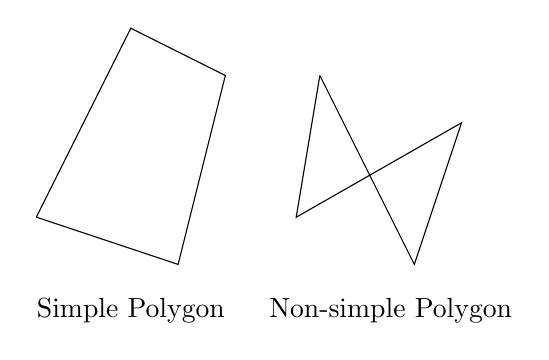
\begin{tikzpicture}[scale=0.6]
					\draw (0, 0) -- (3, -1) -- (4, 3) -- (2, 4) -- (0, 0);
					\draw (6, 3) -- (8, -1) -- (9, 2) -- (5.5, 0) -- (6, 3);
					\node at (2, -1.5) [below] {Simple Polygon};
					\node at (7.5, -1.5) [below] {Non-simple Polygon};
				\end{tikzpicture}
			\end{figure}

			Polygons are basic building blocks in most geometric applications. It can model arbitrarily complex shapes, and apply simple algorithms and algebraic representation/manipulation.
			
		\section{Triangulation}
			\begin{definition}[Triangulation]
				\textbf{Triangulation} is to partition polygon $P$ into non-overlapping triangles using diagonals only. It reduces complex shapes to collection of simpler shapes. Every simple $n$-gon admits a triangulation which has $n-2$ triangles.				
			\end{definition}

			\begin{figure}[h!]
				\centering
				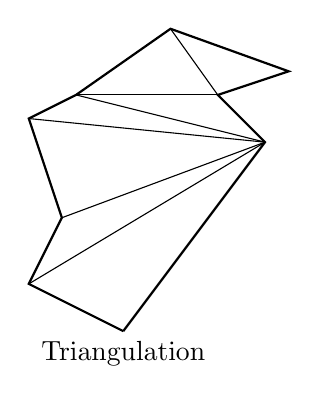
\begin{tikzpicture}[scale=0.6]
					\draw [thick] (0, 0) -- (3, 4) -- (2, 5) -- (3.5, 5.5) -- (1, 6.4) -- (-1, 5) -- (-2, 4.5) -- (-1.3, 2.4) -- (-2, 1) -- (0, 0);
					\draw (-2, 1) -- (3, 4);
					\draw (-1.3, 2.4) -- (3, 4);
					\draw (-2, 4.5) -- (3, 4);
					\draw (-1, 5) -- (3, 4);
					\draw (-1, 5) -- (2, 5);
					\draw (2, 5) -- (1, 6.4);
					\node at (0, 0) [below] {Triangulation};
				\end{tikzpicture}
			\end{figure}

			\begin{theorem}
				Every polygon has a triangulation				
			\end{theorem}

			\begin{lemma}
				Every polygon with more than three vertices has a diagonal.
			\end{lemma}

			\begin{proof}
				(by Meisters, 1975) Let $P$ be a polygon with more than three vertices. Every vertex of a $P$ is either \textit{convex} or \textit{concave}. W.L.O.G.(any polygon must has convex corner) Assume $p$ is a convex vertex. Denote the neighbors of $p$ as $q$ and $r$. If $\bar{qr}$ is a diagonal, done, and we call $\triangle{pqr}$ is an \textit{ear}. If $\triangle{pqr}$ is not an ear, it means at least one vertex is inside $\triangle{pqr}$, assume among those vertexes inside $\triangle{pqr}$, $s$ is a vertex closest to $p$, then $\bar{ps}$ is a diagonal.
			\end{proof}
			
		\section{Art Gallery Theorem}
			\begin{theorem}
				Every $n$-gon can be guarded with $\lfloor \frac{n}{3} \rfloor$ vertex guards
			\end{theorem}

			\begin{lemma}
				Triangulation graph can be 3-colored.
			\end{lemma}

			\begin{problem}
				The floor plan of an art gallery modeled as a simple polygon with $n$ vertices, there are guards which is stationed at fixed positions with 360 degree vision but cannot see through the walls. How many guards does the art gallery need for the security? (Fun fact: This problem was posted to Vasek Chvatal by Victor Klee in 1973).				
			\end{problem}

			\begin{proof}
				- $P$ plus triangulation is a planar graph\\
				- 3-coloring means there exist a 3-partition for vertices that no edge or diagonal has both endpoints within the same set of vertices.\\
				- Proof by Induction:\\
				\indent - Remove an ear (there will always exist ear) \\
				\indent - Inductively 3-color the rest\\
				\indent - Put ear back, coloring new vertex with the label not used by the boundary diagonal.
			\end{proof}

		\section{Triangulation Algorithms}
